


%_______________
\section{Exercises}



%_______________
\subsection{Case study: using stents to prevent strokes}

% 1

\eoce{\qt{Migraine and acupuncture\label{migraine_and_acupuncture_intro}} A migraine 
is a particularly painful type of headache, which patients sometimes wish to 
treat with acupuncture. To determine whether acupuncture relieves migraine 
pain, researchers conducted a randomized controlled study where 89 females 
diagnosed with migraine headaches were randomly assigned to one of two groups: 
treatment or control. 43 patients in the treatment group received acupuncture 
that is specifically designed to treat migraines. 46 patients in the control 
group received placebo acupuncture (needle insertion at non-acupoint 
locations). 24 hours after patients received acupuncture, they were asked 
if they were pain free. Results are summarized in the contingency table below. 
\footfullcite{Allais:2011}

\noindent\begin{minipage}[l]{0.4\textwidth}
\begin{tabular}{ll  cc c} 
			                         &           & \multicolumn{2}{c}{\textit{Pain free}} \\
\cline{3-4}
			                         &			 & Yes 	    & No 	                      & Total	\\
\cline{2-5}
							         & Treatment & 10	 	& 33		                  & 43 	\\
\raisebox{1.5ex}[0pt]{\emph{Group}}  & Control	 & 2	 	& 44 	 	                  & 46 \\
\cline{2-5}
							         &Total		 & 12		& 77		                  & 89
\end{tabular}
\end{minipage}
\begin{minipage}[c]{0.05\textwidth}
\end{minipage}
\begin{minipage}[c]{0.27\textwidth}
\begin{center}
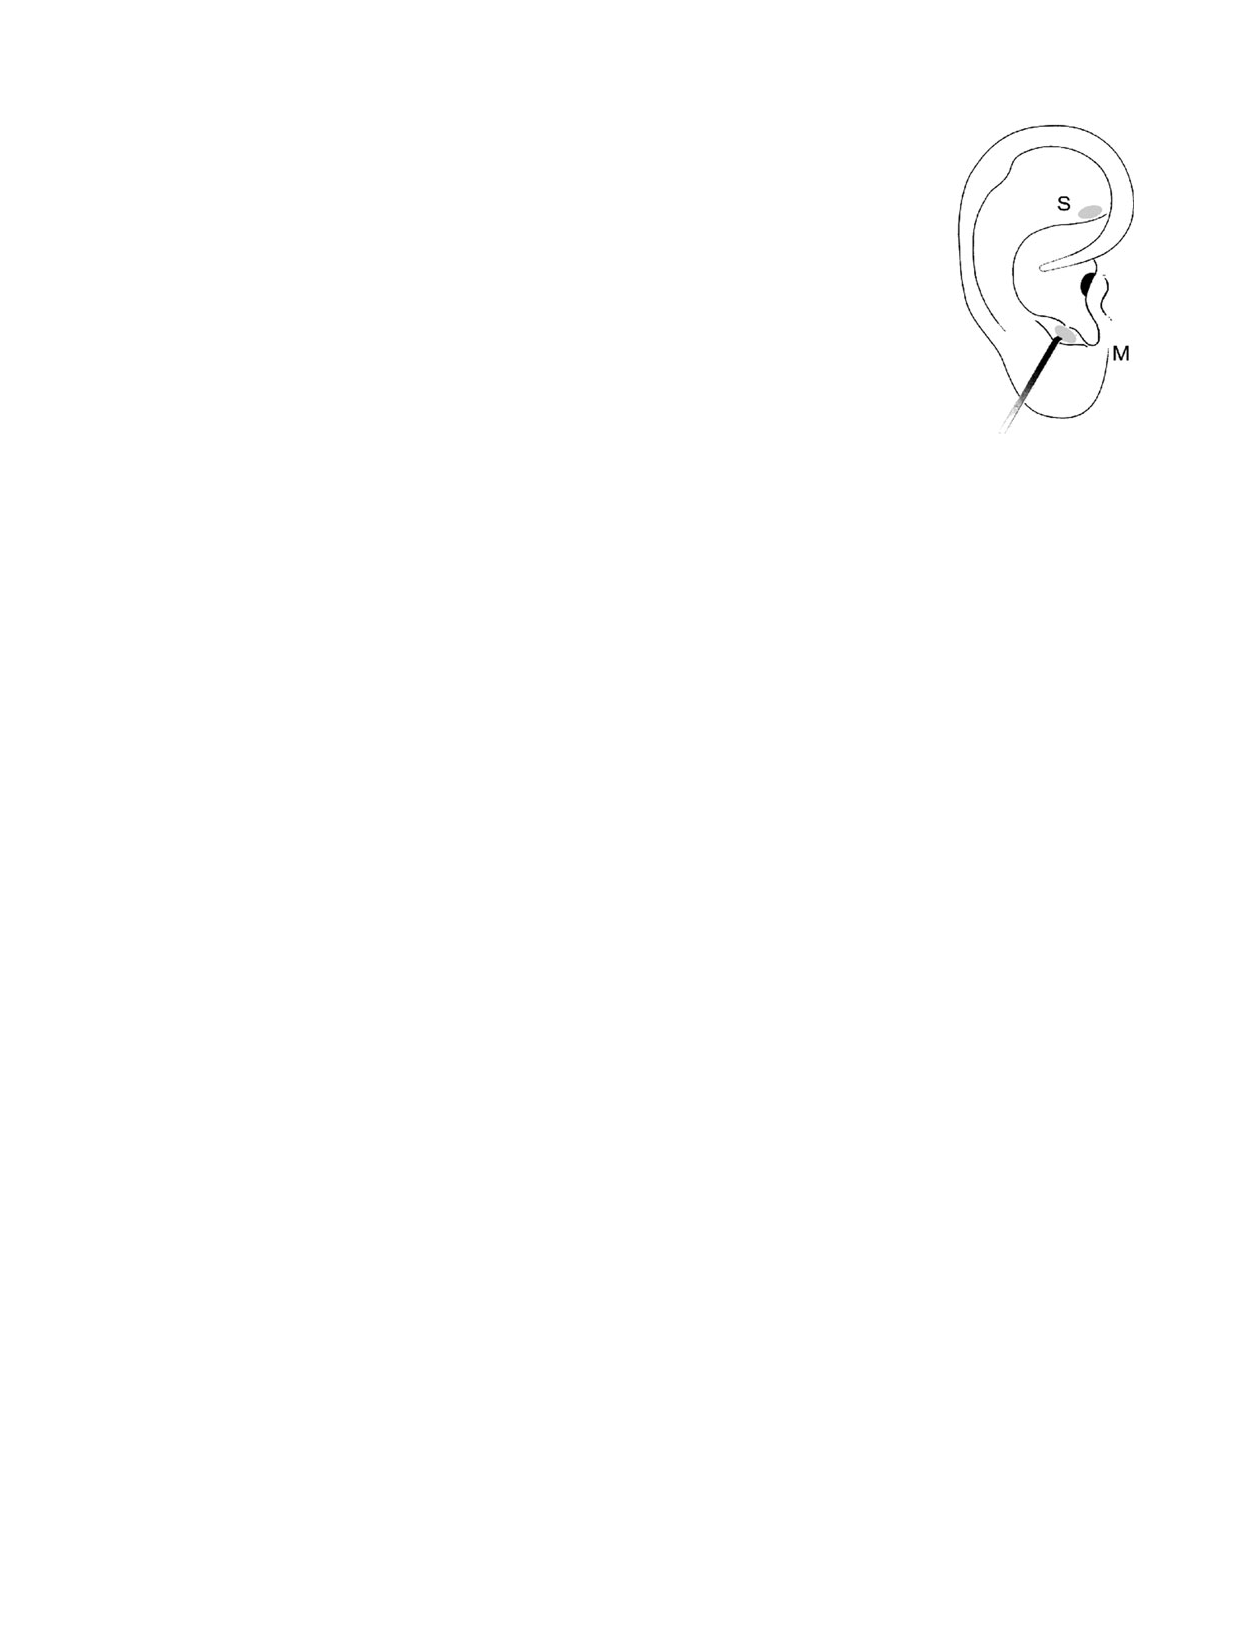
\includegraphics[width = 0.75\textwidth]{ch_intro_to_data/figures/eoce/migraine_and_acupuncture_intro/earacupuncture.pdf}
\end{center}
\end{minipage}
\begin{minipage}[c]{0.25\textwidth}
{\footnotesize Figure from the original paper displaying the appropriate area 
(M) versus the inappropriate area (S) used in the treatment of migraine attacks.}
\end{minipage}
\begin{parts}
\item What percent of patients in the treatment group were pain free 24 hours 
after receiving acupuncture? What percent in the control group?
\item At first glance, does acupuncture appear to be an effective treatment for 
migraines? Explain your reasoning.
\item Do the data provide convincing evidence that there is a real pain reduction 
for those patients in the treatment group? Or do you think that the observed 
difference might just be due to chance?
\end{parts}
}{}

% 2

\eoce{\qt{Sinusitis and antibiotics\label{sinusitis_and_antibiotics_intro}} 
Researchers studying the effect of antibiotic treatment for acute sinusitis 
compared to symptomatic treatments randomly assigned 166 adults diagnosed 
with acute sinusitis to one of two groups: treatment or control. Study 
participants received either a 10-day course of amoxicillin (an antibiotic) 
or a placebo similar in appearance and taste. The placebo consisted of 
symptomatic treatments such as acetaminophen, nasal decongestants, etc. At the 
end of the 10-day period patients were asked if they experienced significant 
improvement in symptoms. The distribution of responses are summarized below. 
\footfullcite{Garbutt:2012}
\begin{center}
\begin{tabular}{ll  cc c} 
                                    &			& \multicolumn{2}{c}{\textit{Self-reported significant}} \\
			                        &			& \multicolumn{2}{c}{\textit{improvement in symptoms}} \\
\cline{3-4}
			                        &			& Yes 	& No 	& Total	\\
\cline{2-5}
							        & Treatment & 66	& 19	& 85 \\
\raisebox{1.5ex}[0pt]{\emph{Group}}	& Control	& 65	& 16 	& 81 \\
\cline{2-5}
							        & Total		& 131	& 35	& 166
\end{tabular}
\end{center}
\begin{parts}
\item What percent of patients in the treatment group experienced a significant 
improvement in symptoms? What percent in the control group?
\item Based on your findings in part (a), which treatment appears to be more 
effective for sinusitis?
\item Do the data provide convincing evidence that there is a difference in the 
improvement rates of sinusitis symptoms? Or do you think that the observed 
difference might just be due to chance?
\end{parts}
}{}



%_______________
\subsection{Data basics}

% 3

\eoce{\qt{Air pollution and birth outcomes, study components\label{study_components_airpoll}} 
Researchers collected data to examine the relationship between air pollutants 
and preterm births in Southern California. During the study air pollution levels 
were measured by air quality monitoring stations. Specifically, levels of carbon 
monoxide were recorded in parts per million, nitrogen dioxide and ozone in parts 
per hundred million, and coarse particulate matter (PM$_{10}$) in $\mu g/m^3$. 
Length of gestation data were collected on 143,196 births between the years 1989 
and 1993, and air pollution exposure during gestation was calculated for each 
birth. The analysis suggested that increased ambient PM$_{10}$ and, to a lesser 
degree, CO concentrations may be associated with the occurrence of preterm births. 
\footfullcite{Ritz+Yu+Chapa+Fruin:2000}. Identify
\begin{parts}
\item the cases,
\item the variables and their types, and
\item the main research question 
\end{parts}
in this study.
}{}

% 4

\eoce{\qt{Buteyko method, study components\label{study_components_buteyko}} 
The Buteyko method is a shallow breathing technique developed by Konstantin 
Buteyko, a Russian doctor, in 1952. Anecdotal evidence suggests that the Buteyko 
method can reduce asthma symptoms and improve quality of life. In a scientific 
study to determine the effectiveness of this method, researchers recruited 600 
asthma patients aged 18-69 who relied on medication for asthma treatment. These 
patients were split into two research groups: one practiced the Buteyko method 
and the other did not. Patients were scored on quality of life, activity, 
asthma symptoms, and medication reduction on a scale from 0 to 10. On average, 
the participants in the Buteyko group experienced a significant reduction in 
asthma symptoms and an improvement in quality of life. \footfullcite{McDowan:2003}. 
Identify
\begin{parts}
\item the cases,
\item the variables and their types, and
\item the main research question 
\end{parts}
in this study.
}{}

% 5

\eoce{\qt{Cheaters, study components\label{study_components_cheaters}} 
Researchers studying the relationship between honesty, age and 
self-control conducted an experiment on 160 children between the ages of 5 and 
15. Participants reported their age, sex, and whether they were an only child 
or not. The researchers asked each child to toss a fair coin in private and 
to record the outcome (white or black) on a paper sheet, and said they 
would only reward children who report white. Half the students were explicitly 
told not to cheat and the others were not given any explicit instructions. In 
the no instruction group probability of cheating was found to be uniform 
across groups based on child's characteristics. In the group that was 
explicitly told to not cheat, girls were less likely to cheat, and while rate 
of cheating didn't vary by age for boys, it decreased with age for girls. 
\footfullcite{Bucciol:2011} Identify
\begin{parts}
\item the cases,
\item the variables and their types, and
\item the main research question 
\end{parts}
in this study.
}{}

\textC{\pagebreak}

% 6

\eoce{\qt{Stealers, study components\label{study_components_stealers}} 
In a study of the relationship between socio-economic class and unethical 
behavior, 129 University of California undergraduates at Berkeley were asked 
to identify themselves as having low or high social-class by comparing 
themselves to others with the most (least) money, most (least) education, and 
most (least) respected jobs. They were also presented  with a jar of 
individually wrapped candies and informed that the candies were for children
in a nearby laboratory, but that they could take some if they wanted. After 
completing some unrelated tasks, participants reported the number of candies 
they had taken. It was found that those who were identified as upper-class 
took more candy than others. \footfullcite{Piff:2012} Identify
\begin{parts}
\item the cases,
\item the variables and their types, and
\item the main research question 
\end{parts}
in this study.
}{}

% 7

\eoce{\qt{Fisher's irises\label{fisher_irises}} Sir Ronald Aylmer Fisher was an 
English statistician, evolutionary biologist, and geneticist who worked on a 
data set that contained sepal length and width, and petal length and width from 
three species of iris flowers (\textit{setosa}, \textit{versicolor} and 
\textit{virginica}). There were 50 flowers from each species in the data set. 
\footfullcite{Fisher:1936} \\
\noindent\begin{minipage}[c]{0.48\textwidth}
\begin{parts}
\item How many cases were included in the data?
\item How many numerical variables are included in the data? Indicate what 
they are, and if they are continuous or discrete.
\item How many categorical variables are included in the data, and what are 
they? List the corresponding levels (categories).
\end{parts}
\vfill \ 
\end{minipage}
\begin{minipage}[c]{0.01\textwidth}
\ 
\end{minipage}
\begin{minipage}[c]{0.2\textwidth}
\begin{center}
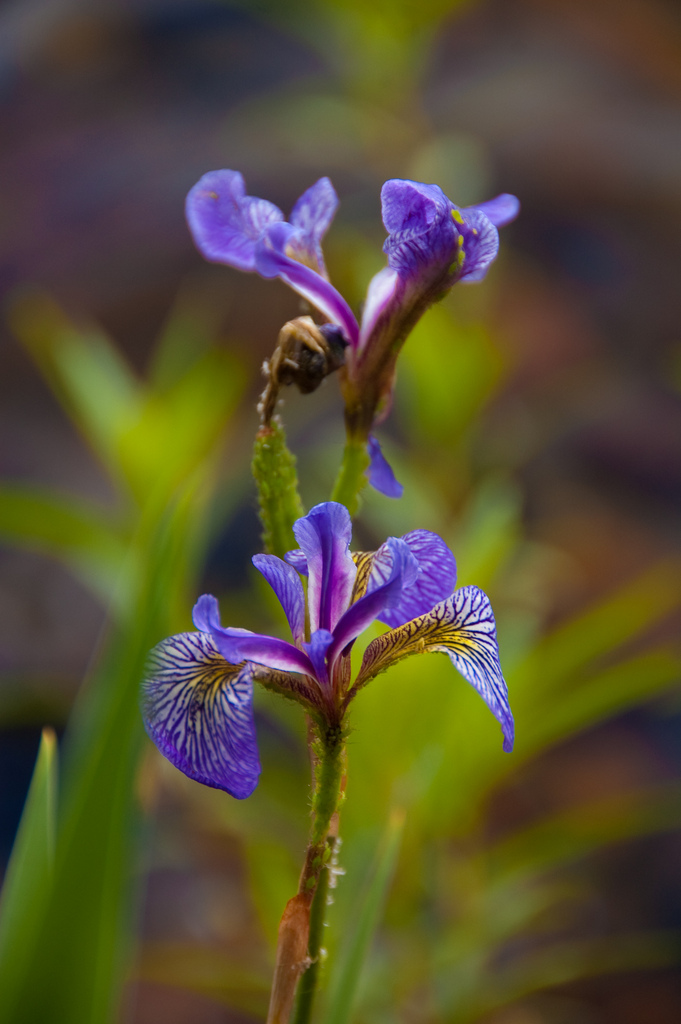
\includegraphics[width = \textwidth]{ch_intro_to_data/figures/eoce/fisher_irises/irisversicolor.jpg}
\end{center}
\end{minipage}
\begin{minipage}[c]{0.01\textwidth}
\ 
\end{minipage}
\begin{minipage}[c]{0.23\textwidth}
{\raggedright\footnotesize Photo by Ryan Claussen 
(\oiRedirect{textbook-flickr_ryan_claussen_iris_picture}{http://flic.kr/p/6QTcuX}) 
\oiRedirect{textbook-CC_BY_SA_2}{CC~BY-SA~2.0~license}}
\vfill \ 
\end{minipage}
}{}

% 8

\eoce{\qt{Smoking habits of UK residents\label{smoking_habits_UK_datamatrix}} A survey 
was conducted to study the smoking habits of UK residents. Below is a data 
matrix displaying a portion of the data collected in this survey. Note that 
``$\pounds$" stands for British Pounds Sterling, ``cig" stands for cigarettes, 
and ``N/A'' refers to a missing component of the data. \footfullcite{data:smoking}
\begin{center}
\scriptsize{
\begin{tabular}{rccccccc}
\hline
	& sex 	 & age 	& marital 	& grossIncome 					     & smoke & amtWeekends	& amtWeekdays \\ 
\hline
1 	& Female & 42 	& Single 	& Under $\pounds$2,600 			     & Yes 	 & 12 cig/day   & 12 cig/day \\ 
2 	& Male	 & 44	& Single 	& $\pounds$10,400 to $\pounds$15,600 & No	 & N/A 			& N/A \\ 
3 	& Male 	 & 53 	& Married   & Above $\pounds$36,400 		     & Yes 	 & 6 cig/day 	& 6 cig/day \\ 
\vdots & \vdots & \vdots & \vdots & \vdots 				             & \vdots & \vdots 	    & \vdots \\ 
1691 & Male  & 40   & Single 	& $\pounds$2,600 to $\pounds$5,200   & Yes 	 & 8 cig/day 	& 8 cig/day \\   
\hline
\end{tabular}
}
\end{center}
\begin{parts}
\item What does each row of the data matrix represent?
\item How many participants were included in the survey?
\item Indicate whether each variable in the study is numerical or categorical. If numerical, identify as 
continuous or discrete. If categorical, indicate if the variable is ordinal.
\end{parts}
}{}



\textC{\newpage}

%_______________
\subsection{Overview of data collection principles}

% 9

\eoce{\qt{Air pollution and birth outcomes, scope of inference\label{scope_airpoll}} 
Exercise~\ref{study_components_airpoll} introduces a study where researchers 
collected data to examine the relationship between air pollutants and preterm 
births in Southern California. During the study air pollution levels were 
measured by air quality monitoring stations. Length of gestation data were 
collected on 143,196 births between the years 1989 and 1993, and air pollution 
exposure during gestation was calculated for each birth.
\begin{parts}
\item Identify the population of interest and the sample in this study.
\item Comment on whether or not the results of the study can be generalized to the 
population, and if the findings of the study can be used to establish causal relationships.
\end{parts}
}{}

% 10

\eoce{\qt{Cheaters, scope of inference\label{scope_cheaters}} 
Exercise~\ref{study_components_cheaters} introduces a study where researchers 
studying the relationship between honesty, age, and self-control conducted an 
experiment on 160 children between the ages of 5 and 15. The researchers asked 
each child to toss a fair coin in private and to record the outcome (white or black) 
on a paper sheet, and said they would only reward children who report white. 
Half the students were explicitly told not to cheat and the others were not given 
any explicit instructions. Differences were observed in the cheating rates in the
instruction and no instruction groups, as well as some differences across 
children's characteristics within each group.
\begin{parts}
\item Identify the population of interest and the sample in this study.
\item Comment on whether or not the results of the study can be generalized to the 
population, and if the findings of the study can be used to establish causal 
relationships.
\end{parts}
}{}

% 11

\eoce{\qt{Buteyko method, scope of inference\label{scope_buteyko}} 
Exercise~\ref{study_components_buteyko} introduces a study on using the Buteyko 
shallow breathing technique to reduce asthma symptoms and improve quality of life.
As part of this study 600 asthma patients aged 18-69 who relied on medication for 
asthma treatment were recruited and randomly assigned to two groups: one practiced 
the Buteyko method and the other did not. Those in the Buteyko group experienced,
on average, a significant reduction in asthma symptoms and an improvement in quality 
of life.
\begin{parts}
\item Identify the population of interest and the sample in this study.
\item Comment on whether or not the results of the study can be generalized to the 
population, and if the findings of the study can be used to establish causal 
relationships.
\end{parts}
}{}

% 12

\eoce{\qt{Stealers, scope of inference\label{scope_stealers}} 
Exercise~\ref{study_components_stealers} introduces a study on the relationship 
between socio-economic class and unethical behavior. As part of this study 129 
University of California Berkeley undergraduates were asked to identify themselves 
as having low or high social-class by comparing themselves to others with the most 
(least) money, most (least) education, and most (least) respected jobs. They were 
also presented  with a jar of individually wrapped candies and informed that the
candies were for children in a nearby laboratory, but that they could take some if 
they wanted. After completing some unrelated tasks, participants reported the 
number of candies they had taken. It was found that those who were identified as 
upper-class took more candy than others.
\begin{parts}
\item Identify the population of interest and the sample in this study.
\item Comment on whether or not the results of the study can be generalized to the 
population, and if the findings of the study can be used to establish causal 
relationships.
\end{parts}
}{}

\textC{\newpage}

% 13

\eoce{\qt{Relaxing after work\label{relax_after_work_definitions}} The 2010 General 
Social Survey asked the question, ``After an average work day, about how many 
hours do you have to relax or pursue activities that you enjoy?" to a random 
sample of 1,155 Americans. The average relaxing time was found to be 1.65 
hours. Determine which of the following is an observation, a variable, a 
sample statistic, or a population parameter.
\begin{parts}
\item An American in the sample.
\item Number of hours spent relaxing after an average work day.
\item 1.65.
\item Average number of hours all Americans spend relaxing after an average 
work day.
\end{parts}
}{}

% 14

\eoce{\qt{Cats on YouTube\label{cats_on_youtube_definitions}} Suppose you want to 
estimate the percentage of videos on YouTube that are cat videos. It is 
impossible for you to watch all videos on YouTube so you use a random video 
picker to select 1000 videos for you. You find that 2\% of these videos are 
cat videos.Determine which of the following is an observation, a variable, 
a sample statistic, or a population parameter.
\begin{parts}
\item Percentage of all videos on YouTube that are cat videos.
\item 2\%.
\item A video in your sample.
\item Whether or not a video is a cat video.
\end{parts}
}{}

% 15

\eoce{\qt{GPA and study hours\label{gpa_study_hours}} A survey was conducted on 193 
Duke University undergraduates who took an introductory statistics course in 
2012. Among many other questions, this survey asked them about their GPA, which 
can range between 0 and 4 points, and the number of hours they spent studying 
per week. The scatterplot below displays the relationship between these two 
variables.

\noindent\begin{minipage}[c]{0.44\textwidth}
\begin{parts}
\item What is the explanatory variable and what is the response variable?
\item Describe the relationship between the two variables. Make sure to discuss 
unusual observations, if any.
\item Is this an experiment or an observational study?
\item Can we conclude that studying longer hours leads to higher GPAs?
\end{parts}
\end{minipage}
\begin{minipage}[c]{0.55\textwidth}
\begin{center}
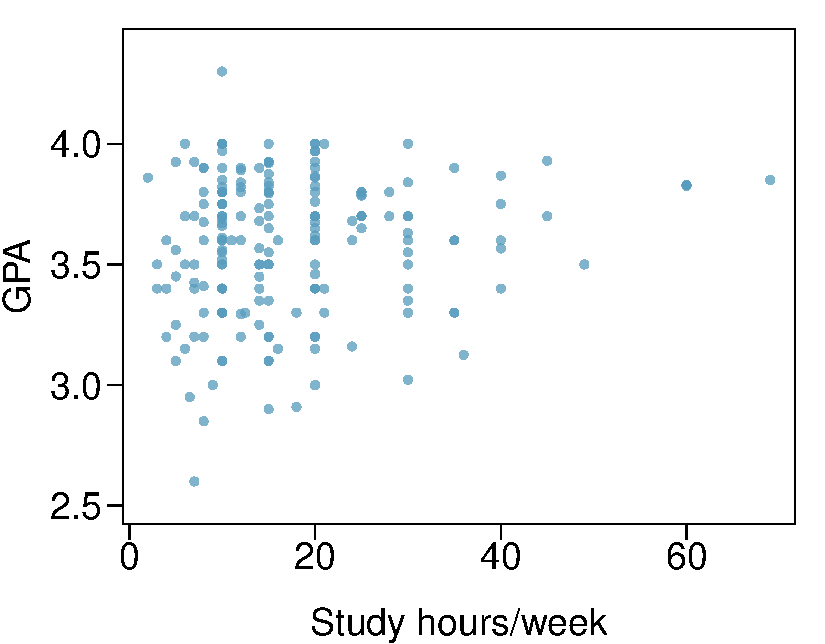
\includegraphics[width = 0.78\textwidth]{ch_intro_to_data/figures/eoce/gpa_study_hours/gpa_study_hours_scatterplot.pdf}
\end{center}
\end{minipage}
}{}

% 16

\eoce{\qt{Income and education in US counties\label{income_education_county}} 
The scatterplot below shows the relationship between per capita income 
(in thousands of dollars) and percent of population with a bachelor's 
degree in 3,143 counties in the US in 2010.

\noindent\begin{minipage}[c]{0.44\textwidth}
\begin{parts}
\item What are the explanatory and response variables?
\item Describe the relationship between the two variables. Make sure to discuss 
unusual observations, if any.
\item Can we conclude that having a bachelor's degree increases one's income?
\end{parts} \vspace{8mm}
\end{minipage}
\begin{minipage}[c]{0.55\textwidth}
\begin{center}
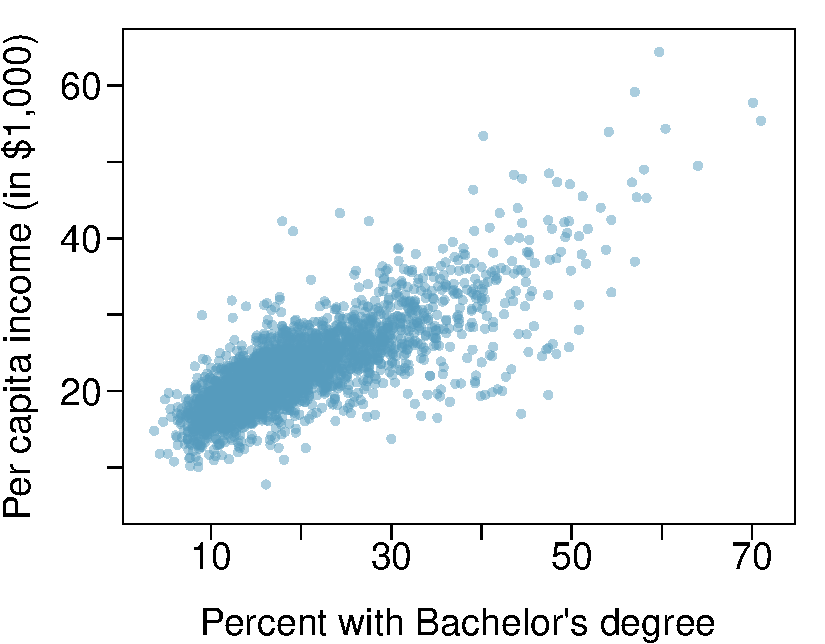
\includegraphics[width = 0.78\textwidth]{ch_intro_to_data/figures/eoce/county_income_education/county_income_education_scatterplot.pdf}
\end{center}
\end{minipage}
}{}



%_______________
\subsection{Observational studies and sampling strategies}

% 17

\eoce{\qt{Course satisfaction across sections\label{course_satisfaction_sections}} 
A large college class has 160 students. All 160 students attend the lectures 
together, but the students are divided into 4 groups, each of 40 students, 
for lab sections administered by different teaching assistants. The professor 
wants to conduct a survey about how satisfied the students are with the course, 
and he believes that the lab section a student is in might affect the student's 
overall satisfaction with the course.
\begin{parts}
\item What type of study is this?
\item Suggest a sampling strategy for carrying out this study.
\end{parts}
}{}

% 18

\eoce{\qt{Housing proposal across dorms\label{housing_proposal_dorms}} On a large 
college campus first-year students and sophomores live in dorms located on 
the eastern part of the campus and juniors and seniors live in dorms located 
on the western part of the campus. Suppose you want to collect student opinions 
on a new housing structure the college administration is proposing and you want 
to make sure your survey equally represents opinions from students from all years.
\begin{parts}
\item What type of study is this?
\item Suggest a sampling strategy for carrying out this study.
\end{parts}
}{}

% 19

\eoce{\qt{Internet use and life expectancy\label{internet_life_expactancy}} The 
following scatterplot was created as part of a study evaluating the 
relationship between estimated life expectancy at birth (as of 2014) and 
percentage of internet users (as of 2009) in 208 countries for which such 
data were available.\footfullcite{data:ciaFactbook}

\noindent\begin{minipage}[c]{0.44\textwidth}
\begin{parts}
\item Describe the relationship between life expectancy and percentage of 
internet users.
\item What type of study is this?
\item State a possible confounding variable that might explain this relationship 
and describe its potential effect.
\end{parts} \vspace{15mm}
\end{minipage}
\begin{minipage}[r]{0.55\textwidth}
\hfill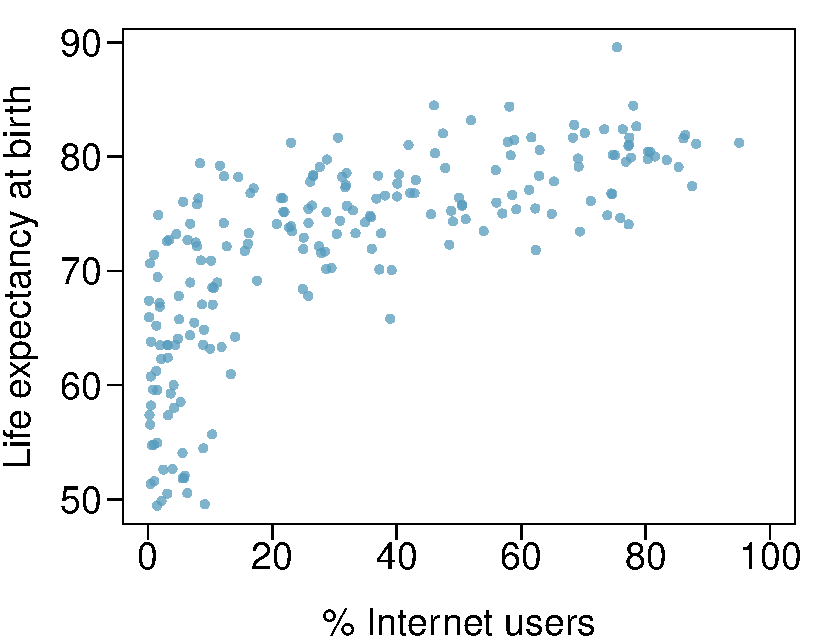
\includegraphics[width = 0.87\textwidth]{ch_intro_to_data/figures/eoce/internet_life_expactancy/internet_life_expactancy.pdf}
\end{minipage}
}{}

% 20

\eoce{\qt{Stressed out, Part I\label{stressed_out_observational}} A study that 
surveyed a random sample of otherwise healthy high school students found that 
they are more likely to get muscle cramps when they are stressed. The study 
also noted that students drink more coffee and sleep less when they are 
stressed.
\begin{parts}
\item What type of study is this?
\item Can this study be used to conclude a causal relationship between 
increased stress and muscle cramps?
\item State possible confounding variables that might explain the observed 
relationship between increased stress and muscle cramps. 
\end{parts}
}{}

% 21

\eoce{\qt{Evaluate sampling methods\label{evaluate_sampling_methods}}
A university wants to determine what fraction of its undergraduate 
student body support a new \$25 annual fee to improve the student 
union. For each proposed method below, indicate whether the method 
is reasonable or not.
\begin{parts}
\item Survey a simple random sample of 500 students.
\item Stratify students by their field of study, then sample 10\% of 
students from each stratum.
\item Cluster students by their ages (e.g. 18 years old in one 
cluster, 19 years old in one cluster, etc.), then randomly sample 
three clusters and survey all students in those clusters.
\end{parts}}{}

\textC{\pagebreak}

% 22

\eoce{\qt{Random digit dialing\label{random_digit_dialing}} The Gallup Poll uses a 
procedure called random digit dialing, which creates phone numbers based on 
a list of all area codes in America in conjunction with the associated number 
of residential households in each area code. Give a possible reason the Gallup 
Poll chooses to use random digit dialing instead of picking phone numbers 
from the phone book.
}{}

% 23

\eoce{\qt{Haters are gonna hate, study confirms\label{scope_haters}} A study 
published in the \textit{Journal of Personality and Social Psychology} asked a 
group of 200 randomly sampled men and women to evaluate how they felt about 
various subjects, such as camping, health care, architecture, taxidermy, 
crossword puzzles, and Japan in order to measure their dispositional attitude 
towards mostly independent stimuli. Then, they presented the participants with 
information about a new product: a microwave oven. This microwave oven does 
not exist, but the participants didn't know this, and were given three 
positive and three negative fake reviews. People who reacted positively to the 
subjects on the dispositional attitude measurement also tended to react 
positively to the microwave oven, and those who reacted negatively also tended 
to react negatively to it. Researchers concluded that ``some people tend to 
like things, whereas others tend to dislike things, and a more thorough 
understanding of this tendency will lead to a more thorough understanding of 
the psychology of attitudes." \footfullcite{Hepler:2013}
\begin{parts}
\item What are the cases?
\item What is (are) the response variable(s) in this study?
\item What is (are) the explanatory variable(s) in this study?
\item Does the study employ random sampling?
\item Is this an observational study or an experiment? Explain your reasoning.
\item Can we establish a causal link between the explanatory and response 
variables?
\item Can the results of the study be generalized to the population at large?
\end{parts}
}{}

% 24

\eoce{\qt{Family size\label{family_size}} Suppose we want to estimate household 
size, where a ``household" is defined as people living together in the 
same dwelling, and sharing living accommodations. If we select students 
at random at an elementary school and ask them what their family size is, 
will this be a good measure of household size? Or will our average be 
biased? If so, will it overestimate or underestimate the true value?
}{}

% 25

\eoce{\qt{Flawed reasoning\label{flawed_reasoning}} Identify the flaw(s) in reasoning 
in the following scenarios. Explain what the individuals in the study should 
have done differently if they wanted to make such strong conclusions.
\begin{parts}
\item Students at an elementary school are given a questionnaire that they 
are asked to return after their parents have completed it. One of the questions 
asked is, ``Do you find that your work schedule makes it difficult for you to 
spend time with your kids after school?" Of the parents who replied, 85\% said 
``no". Based on these results, the school officials conclude that a great 
majority of the parents have no difficulty spending time with their kids 
after school.
\item A survey is conducted on a simple random sample of 1,000 women who 
recently gave birth, asking them about whether or not they smoked during 
pregnancy. A follow-up survey asking if the children have respiratory problems 
is conducted 3 years later, however, only 567 of these women are reached at the 
same address. The researcher reports that these 567 women are representative 
of all mothers.
\item A orthopedist administers a questionnaire to 30 of his patients who do 
not have any joint problems and finds that 20 of them regularly go running. 
He concludes that running decreases the risk of joint problems.
\end{parts}
}{}

\textC{\pagebreak}

% 26

\eoce{\qt{City council survey\label{city_council_survey}} A city council has requested a 
household survey be conducted in a suburban area of their city. The area is broken 
into many distinct and unique neighborhoods, some including large homes, some with 
only apartments, and others a diverse mixture of housing structures. Identify the 
sampling methods described below, and comment on whether or not you think they 
would be effective in this setting.
\begin{parts}
\item Randomly sample 50 households from the city.
\item Divide the city into neighborhoods, and sample 20 households from each 
neighborhood.
\item Divide the city into neighborhoods, randomly sample 10 neighborhoods, 
and sample all households from those neighborhoods.
\item Divide the city into neighborhoods, randomly sample 10 neighborhoods, 
and then randomly sample 20 households from those neighborhoods.
\item Sample the 200 households closest to the city council offices.
\end{parts}
}{}

% 27

\eoce{\qt{Sampling strategies\label{sampling_strategies}} A statistics student who is curious about the relationship between the amount of time students spend on social networking sites and their performance at school decides to conduct a survey. Various research strategies for collecting data are described below. In each, name the sampling method proposed and any bias you might expect.
\begin{parts}
\item He randomly samples 40 students from the study's population, gives them the survey, asks them to fill it out and bring it back the next day.
\item He gives out the survey only to his friends, making sure each one of them fills out the survey.
\item He posts a link to an online survey on Facebook and asks his friends to fill out the survey.
\item He randomly samples 5 classes and asks a random sample of students from those classes to fill out the survey.
\end{parts}
}{}

% 28

\eoce{\qt{Reading the paper\label{reading_paper}} Below are excerpts from two 
articles published in the \emph{NY Times}:
\begin{parts}
\item An article titled \emph{Risks: Smokers Found More Prone to Dementia} 
states the following: \footfullcite{news:smokingDementia}
\begin{adjustwidth}{1em}{1em}
{\footnotesize ``Researchers analyzed data from 23,123 health plan members who 
participated in a voluntary exam and health behavior survey from 1978 to 1985, 
when they were 50-60 years old. 23 years later, about 25\% of the group had 
dementia, including 1,136 with Alzheimer's disease and 416 with vascular 
dementia. After adjusting for other factors, the researchers concluded that 
pack-a-day smokers were 37\% more likely than nonsmokers to develop dementia, 
and the risks went up with increased smoking; 44\% for one to two packs a day; 
and twice the risk for more than two packs."}
\end{adjustwidth}
Based on this study, can we conclude that smoking causes dementia later in 
life? Explain your reasoning.
\item Another article titled \emph{The School Bully Is Sleepy} states the 
following: \footfullcite{news:bullySleep}
\begin{adjustwidth}{1em}{1em}
{\footnotesize ``The University of Michigan study, collected survey data from 
parents on each child's sleep habits and asked both parents and teachers to 
assess behavioral concerns. About a third of the students studied were 
identified by parents or teachers as having problems with disruptive behavior 
or bullying. The researchers found that children who had behavioral issues and 
those who were identified as bullies were twice as likely to have shown 
symptoms of sleep disorders."}
\end{adjustwidth}
A friend of yours who read the article says, ``The study shows that sleep 
disorders lead to bullying in school children." Is this statement justified? 
If not, how best can you describe the conclusion that can be drawn from this 
study?
\end{parts}
}{}

\textC{\pagebreak}

% 29

\eoce{\qt{Shyness on Facebook\label{shy_on_fb}} Given the anonymity afforded to 
individuals in online interactions, researchers hypothesized that shy 
individuals might have more favorable attitudes toward Facebook, and that 
shyness might be positively correlated with time spent on Facebook. They also 
hypothesized that shy individuals might have fewer Facebook ``friends" as they 
tend to have fewer friends than non-shy individuals have in the offline world. 
103 undergraduate students at an Ontario university were surveyed via online 
questionnaires. The study states ``Participants were recruited through the  
university's psychology participation pool. After indicating an interest in 
the study, participants were sent an e-mail containing the study's URL." Are 
the results of this study generalizable to the population of all Facebook
users? \footfullcite{Orr:2009}
}{}



%_______________
\subsection{Experiments}

% 30

\eoce{\qt{Stressed out, Part II\label{stressed_out_experiment}} In a study evaluating the 
relationship between stress and muscle cramps half the subjects are randomly assigned to 
be exposed to increased stressed by being placed into an elevator that falls rapidly and 
stops abruptly and the other half are left at no or baseline stress.
\begin{parts}
\item What type of study is this?
\item Can this study be used to conclude a causal relationship between increased stress 
and muscle cramps?
\end{parts}
}{}

% 31

\eoce{\qt{Light and exam performance\label{light_exam_performance}} A study is designed to 
test the effect of light level on exam performance of students. The researcher believes 
that light levels might have different effects on males and females, so wants to make 
sure both are equally represented in each treatment. The treatments are fluorescent 
overhead lighting, yellow overhead lighting, no overhead lighting (only desk lamps). 
\begin{parts}
\item What is the response variable?
\item What is the explanatory variable? What are its levels?
\item What is the blocking variable? What are its levels?
\end{parts}
}{}

% 32

\eoce{\qt{Vitamin supplements\label{vitamin_supplement}} In order to assess the effectiveness 
of taking large doses of vitamin C in reducing the duration of the common cold, 
researchers recruited 400 healthy volunteers from staff and students at a university. A 
quarter of the patients were assigned a placebo, and the rest were evenly divided 
between 1g Vitamin C,  3g Vitamin C, or 3g Vitamin C plus additives to be taken at onset 
of a cold for the following two days. All tablets had identical appearance and packaging.
The nurses who handed the prescribed pills to the patients knew which patient received 
which treatment, but the researchers assessing the patients when they were sick did not. 
No significant differences were observed in any measure of cold duration or severity 
between the four medication groups, and the placebo group had the shortest duration of 
symptoms.\footfullcite{Audera:2001}
\begin{parts}
\item Was this an experiment or an observational study? Why?
\item What are the explanatory and response variables in this study?
\item Were the patients blinded to their treatment?
\item Was this study double-blind?
\item Participants are ultimately able to choose whether or not to use the pills 
prescribed to them. We might expect that not all of them will adhere and take their 
pills. Does this introduce a confounding variable to the study? Explain your reasoning.
\end{parts}
}{}

\textC{\pagebreak}

% 33

\eoce{\qt{Light, noise, and exam performance\label{light_noise_exam_performance}} A study is 
designed to test the effect of light level and noise level on exam performance of 
students. The researcher believes that light and noise levels might have different 
effects on males and females, so wants to make sure both are equally represented in each 
treatment. The light treatments considered are fluorescent overhead lighting, yellow 
overhead lighting, no overhead lighting (only desk lamps). The noise treatments 
considered are no noise,  construction noise, and human chatter noise.
\begin{parts}
\item What is the response variable?
\item How many factors are considered in this study? Identify them, and describe their 
levels.
\item What is the role of the sex variable in this study?
\end{parts}
}{}

% 34

\eoce{\qt{Music and learning\label{music_learning}} You would like to conduct an experiment in 
class to see if students learn better if they study without any music, with music that 
has no lyrics (instrumental), or with music that has lyrics. Briefly outline a design for 
this study.
}{}

% 35

\eoce{\qt{Soda preference\label{soda_preference}} You would like to conduct an experiment in 
class to see if your classmates prefer the taste of regular Coke or Diet Coke. Briefly 
outline a design for this study.
}{}

% 36

\eoce{\qt{Exercise and mental health\label{exercise_mental_health}} A researcher is interested 
in the effects of exercise on mental health and he proposes the following study: Use 
stratified random sampling to ensure representative proportions of 18-30, 31-40 and 41-
55 year olds from the population. Next, randomly assign half the subjects from each age 
group to exercise twice a week, and instruct the rest not to exercise. Conduct a mental 
health exam at the beginning and at the end of the study, and compare the results.
\begin{parts}
\item What type of study is this? 
\item What are the treatment and control groups in this study?
\item Does this study make use of blocking? If so, what is the blocking variable?
\item Does this study make use of blinding?
\item Comment on whether or not the results of the study can be used to establish a 
causal relationship between exercise and mental health, and indicate whether or not the 
conclusions can be generalized to the population at large.
\item Suppose you are given the task of determining if this proposed study should get 
funding. Would you have any reservations about the study proposal?
\end{parts}
}{}

% 37

\eoce{\qt{Chia seeds and weight loss\label{chia_weight_lostt}} Chia Pets -- those terra-cotta 
figurines that sprout fuzzy green hair -- made the chia plant a household name. But chia 
has gained an entirely new reputation as a diet supplement.  In one 2009 study, a team 
of researchers recruited 38 men and divided them randomly into two groups: treatment or 
control. They also recruited 38 women, and they randomly placed half of these 
participants into the treatment group and the other half into the control group. One 
group was given 25 grams of chia seeds twice a day, and the other was given a placebo. 
The subjects volunteered to be a part of the study. After 12 weeks, the scientists found 
no significant difference between the groups in appetite or weight loss. 
\footfullcite{Nieman:2009}
\begin{parts}
\item What type of study is this? 
\item What are the experimental and control treatments in this study?
\item Has blocking been used in this study? If so, what is the blocking variable?
\item Has blinding been used in this study?
\item Comment on whether or not we can make a causal statement, and indicate whether or 
not we can generalize the conclusion to the population at large.
\end{parts}
}{}



%_______________
\subsection{Examining numerical data}

% 38

\eoce{\qt{Mammal life spans\label{mammal_life_spans}} Data were collected on life spans (in 
years) and gestation lengths (in days) for 62 mammals. A scatterplot of life span versus 
length of gestation is shown below. \footfullcite{Allison+Cicchetti:1975}

\noindent\begin{minipage}[c]{0.44\textwidth}
\begin{parts}
\item What type of an association is apparent between life span and length of gestation?
\item What type of an association would you expect to see if the axes of the plot were reversed, i.e. if we plotted length of gestation versus life span?
\item Are life span and length of gestation independent? Explain your reasoning.
\end{parts}\vspace{6mm}
\end{minipage}
\begin{minipage}[c]{0.55\textwidth}
\begin{center}
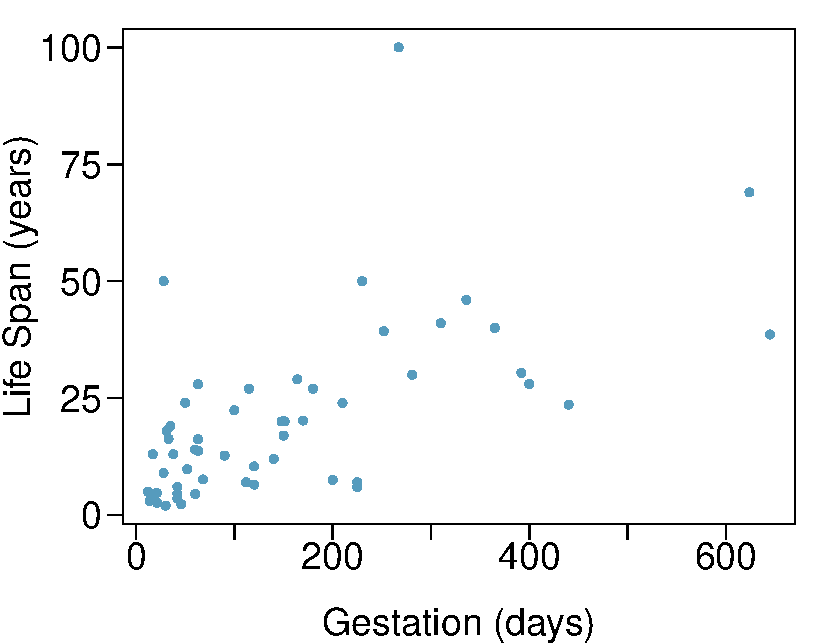
\includegraphics[width = 0.86\textwidth]{ch_intro_to_data/figures/eoce/mammal_life_spans/mammal_life_spans_scatterplot.pdf}
\end{center}
\end{minipage}
}{}

% 39

\eoce{\qt{Associations\label{association_plots}} Indicate which of the plots show a \\[1mm]
\noindent\begin{minipage}[b]{0.35\textwidth}
\begin{parts}
\item positive association
\item negative association
\item no association
\end{parts}
Also determine if the positive and negative associations are linear or nonlinear. Each 
part may refer to more than one plot. \vspace{30mm}
\end{minipage}
\begin{minipage}[b]{0.62\textwidth}
\hfill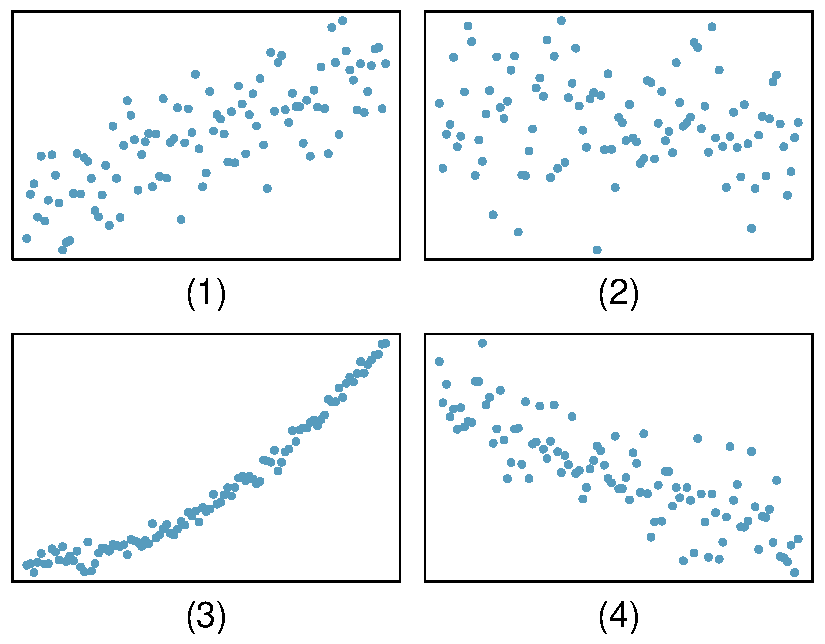
\includegraphics[width = 0.95\textwidth]{ch_intro_to_data/figures/eoce/association_plots/association_plots.pdf}
\end{minipage}
}{}

% 40

\eoce{\qt{Office productivity\label{office_productivity}} Office productivity is relatively low 
when the employees feel no stress about their work or job security. However, high levels 
of stress can also lead to reduced employee productivity. Sketch a plot to represent the 
relationship between stress and productivity.
}{}

% 41

\eoce{\qt{Reproducing bacteria\label{reproducing_bacteria}} Suppose that there is only 
sufficient space and nutrients to support one million bacterial cells in a petri dish. 
You place a few bacterial cells in this petri dish, allow them to reproduce freely, and 
record the number of bacterial cells in the dish over time. Sketch a plot representing 
the relationship between number of bacterial cells and time.
}{}

% 42

\eoce{\qt{Sleeping in college\label{college_sleeping}} A recent article in a college newspaper 
stated that college students get an average of 5.5 hrs of sleep each night. A student who 
was skeptical about this value decided to conduct a survey by randomly sampling 25 
students. On average, the sampled students slept 6.25 hours per night. Identify which 
value represents the sample mean and which value represents the claimed population mean.
}{}

% 43

\eoce{\qt{Parameters and statistics\label{parameters_stats}} Identify which value represents 
the sample mean and which value represents the claimed population mean.
\begin{parts}
\item American households spent an average of about \$52 in 2007 on Halloween 
merchandise such as costumes, decorations and candy. To see if this number had changed, 
researchers conducted a new survey in 2008 before industry numbers were reported. The 
survey included 1,500 households and found that average Halloween spending was \$58 per 
household.
\item The average GPA of students in 2001 at a private university was 3.37. A survey 
on a sample of 203 students from this university yielded an average GPA of 3.59 in 
Spring semester of 2012.
\end{parts}
}{}

% 44

\eoce{\qt{Make-up exam\label{makeup_exam}} In a class of 25 students, 24 of them took an exam 
in class and 1 student took a make-up exam the following day. The professor graded the 
first batch of 24 exams and found an average score of 74 points with a standard 
deviation of 8.9 points. The student who took the make-up the following day scored 64 
points on the exam.
\begin{parts}
\item Does the new student's score increase or decrease the average score?
\item What is the new average?
\item Does the new student's score increase or decrease the standard deviation of the 
scores?
\end{parts}
}{}

% 45

\eoce{\qt{Days off at a mining plant\label{days_off_mining}} Workers at a particular mining 
site receive an average of 35 days paid vacation, which is lower than the national 
average. The manager of this plant is under pressure from a local union to increase the 
amount of paid time off. However, he does not want to give more days off to the workers 
because that would be costly. Instead he decides he should fire 10 employees in such a 
way as to raise the average number of days off that are reported by his employees. In 
order to achieve this goal, should he fire employees who have the most number of days 
off, least number of days off, or those who have about the average number of days off?
}{}

% 46

\eoce{\qt{Medians and IQRs} For each part, compare distributions (1) and (2) based on their medians and IQRs. You do not need to calculate these statistics; simply state how the medians and IQRs compare. Make sure to explain your reasoning. 
\begin{multicols}{2}
\begin{parts}
\item (1) 3, 5, 6, 7, 9 \\
(2) 3, 5, 6, 7, 20
\item (1) 3, 5, 6, 7, 9 \\
(2) 3, 5, 8, 7, 9
\item (1) 1, 2, 3, 4, 5 \\
(2) 6, 7, 8, 9, 10
\item (1) 0, 10, 50, 60, 100 \\
(2) 0, 100, 500, 600, 1000
\end{parts}
\end{multicols}
}{}

% 47

\eoce{\qt{Means and SDs} For each part, compare distributions (1) and (2) based on their means and standard deviations. You do not need to calculate these statistics; simply state how the means and the standard deviations compare. Make sure to explain your reasoning. \textit{Hint:} It may be useful to sketch dot plots of the distributions.
\begin{multicols}{2}
\begin{parts}
\item (1) 3, 5, 5, 5, 8, 11, 11, 11, 13 \\
(2) 3, 5, 5, 5, 8, 11, 11, 11, 20 \\
\item (1) -20, 0, 0, 0, 15, 25, 30, 30 \\
(2) -40, 0, 0, 0, 15, 25, 30, 30
\item (1) 0, 2, 4, 6, 8, 10 \\
(2) 20, 22, 24, 26, 28, 30
\item (1) 100, 200, 300, 400, 500 \\
(2) 0, 50, 300, 550, 600
\end{parts}
\end{multicols}
}{}

% 48

\eoce{\qt{Stats scores\label{stats_scores_box}} Below are the final exam scores of twenty 
introductory statistics students.
\begin{center}
57, 66, 69, 71, 72, 73, 74, 77, 78, 78, 79, 79, 81, 81, 82, 83, 83, 88, 89, 94
\end{center}
Create a box plot of the distribution of these scores. The five number summary provided below may be useful.
\begin{center}
\renewcommand\arraystretch{1.5}
\begin{tabular}{ccccc}
Min & Q1    & Q2 (Median)   & Q3    & Max \\
\hline
57  & 72.5  & 78.5          & 82.5  & 94 \\
\end{tabular}
\end{center}
}{}

% 49

\eoce{\qt{Infant mortality\label{infant_mortality}} The infant mortality rate is defined as 
the number of infant deaths per 1,000 live births. This rate is often used as an 
indicator of the level of health in a country. The relative frequency histogram below 
shows the distribution of estimated infant death rates for 224 countries for which such 
data were available in 2014. 
\footfullcite{data:ciaFactbook}

\noindent\begin{minipage}[c]{0.43\textwidth}
\begin{parts}
\item Estimate Q1, the median, and Q3 from the histogram.
\item Would you expect the mean of this data set to be smaller or larger than the 
median? Explain your reasoning.
\end{parts} \vfill \
\end{minipage}
\begin{minipage}[c]{0.52\textwidth}
\hfill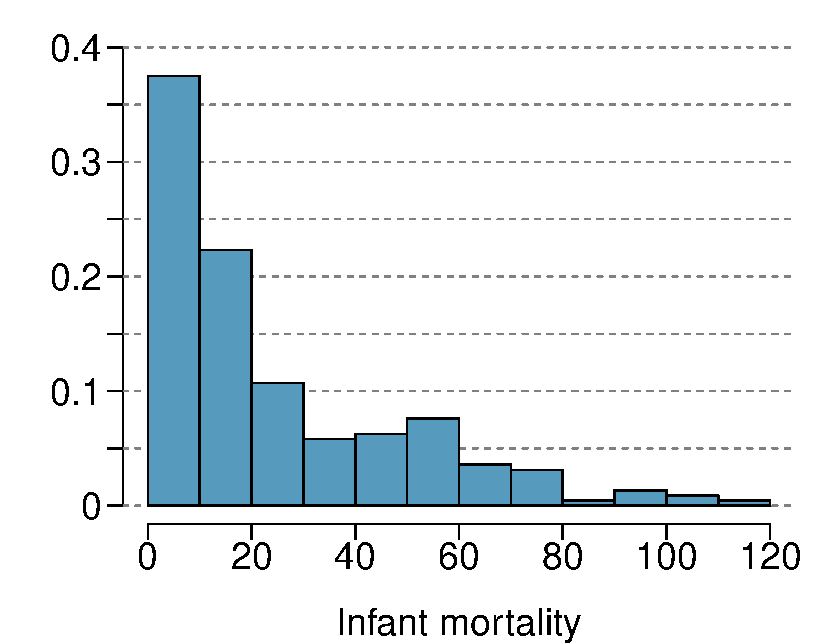
\includegraphics[width = 0.85\textwidth]{ch_intro_to_data/figures/eoce/infant_mortality_rel_freq/infant_mortality_rel_freq_hist.pdf}
\end{minipage}
}{}

% 50

\eoce{\qt{Mix-and-match} Describe the distribution in the histograms below and match them to the box plots. \\
\begin{center}
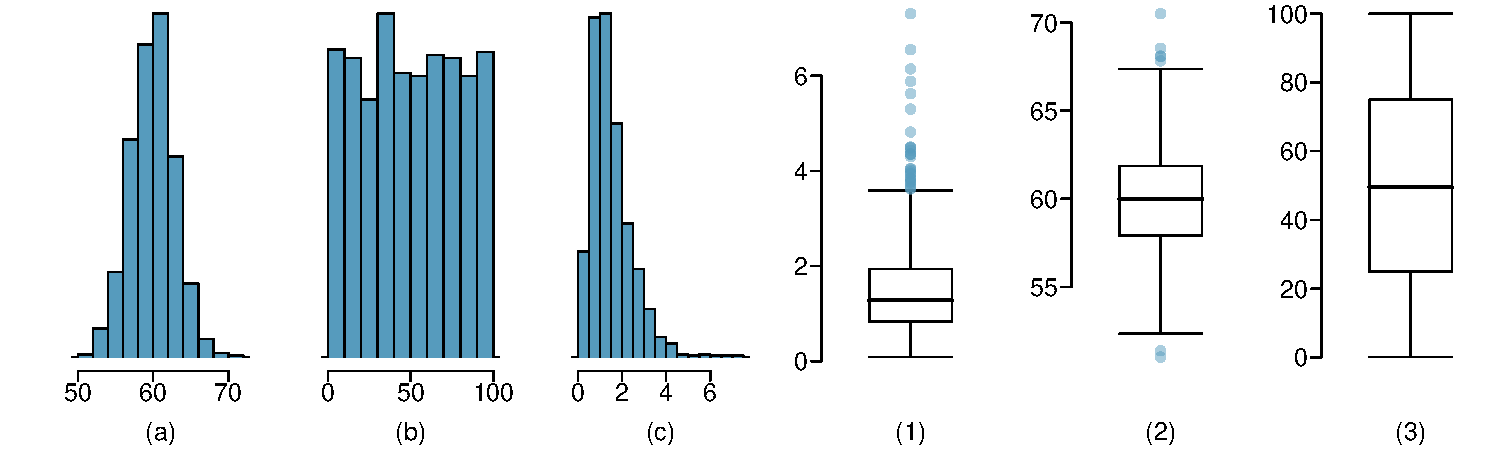
\includegraphics[width=\textwidth]{ch_intro_to_data/figures/eoce/hist_box_match/hist_box_match.pdf}
\end{center}
}{}

% 51

\eoce{\qt{Air quality\label{air_quality_durham}} Daily air quality is measured by the air 
quality index (AQI) reported by the Environmental Protection Agency. This index reports 
the pollution level and what associated health effects might be a concern. The index is 
calculated for five major air pollutants regulated by the Clean Air Act and takes values 
from 0 to 300, where a higher value indicates lower air quality. AQI was reported for a 
sample of 91 days in 2011 in Durham, NC. The relative frequency histogram below shows 
the distribution of the AQI values on these days. \footfullcite{data:durhamAQI:2011}
\begin{minipage}[c]{0.55\textwidth}
\begin{parts}
\item Estimate the median AQI value of this sample.
\item Would you expect the mean AQI value of this sample to be higher or lower than the 
median? Explain your reasoning.
\item Estimate Q1, Q3, and IQR for the distribution.
\item Would any of the days in this sample be considered to have an unusually low or 
high AQI? Explain your reasoning.
\end{parts}
\end{minipage}
\begin{minipage}[c]{0.45\textwidth}
\begin{center}
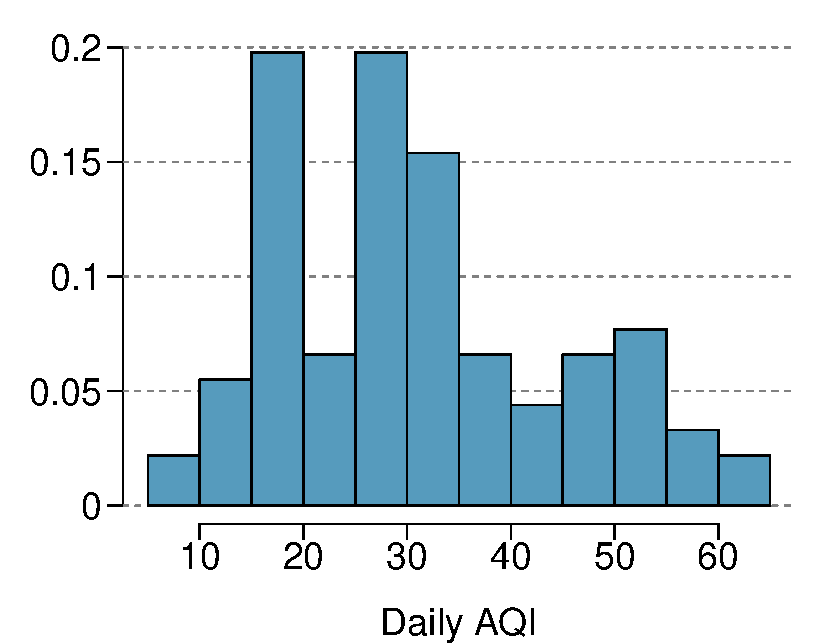
\includegraphics[width = \textwidth]{ch_intro_to_data/figures/eoce/air_quality_durham/air_quality_durham_rel_freq_hist.pdf} 
\end{center}
\end{minipage}
}{}

\textC{\pagebreak}

% 52

\eoce{\qt{Median vs. mean\label{estimate_mean_median_simple}}
Estimate the median for the 400 observations shown in the histogram, and note whether you expect the mean to be higher or lower than the median.
\begin{center}
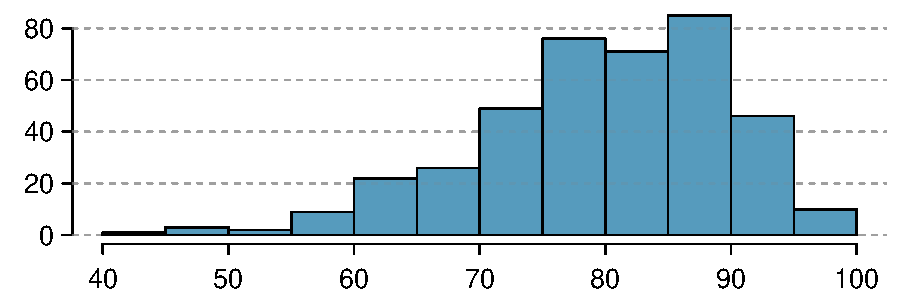
\includegraphics[width = 0.6\textwidth]{ch_intro_to_data/figures/eoce/estimate_mean_median_simple/estimate_mean_median_simple.pdf} 
\end{center}}

% 53

\eoce{\qt{Histograms vs. box plots\label{hist_vs_box}} Compare the two plots below. What 
characteristics of the distribution are apparent in the histogram and not in the box 
plot? What characteristics are apparent in the box plot but not in the histogram?
\begin{center}
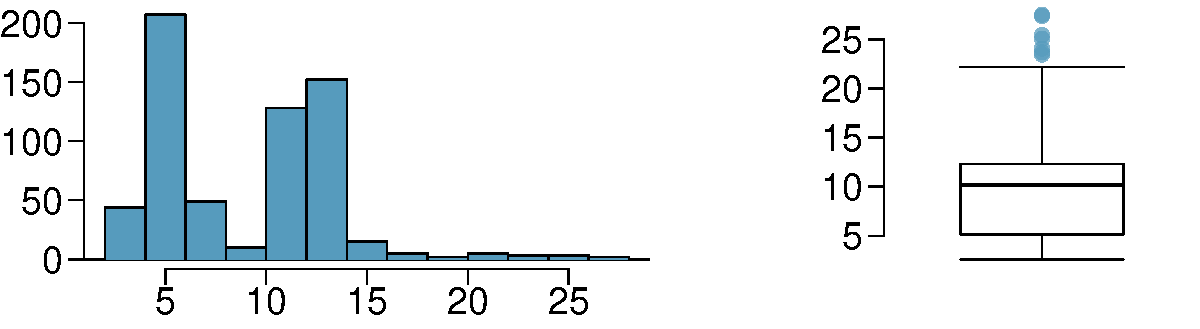
\includegraphics[width = 0.6\textwidth]{ch_intro_to_data/figures/eoce/hist_vs_box/hist_vs_box.pdf}
\end{center}
}{}

% 54

\eoce{\qt{Marathon winners\label{marathon_winners}} The histogram and box plots below show the distribution of finishing times for male and female winners of the New York Marathon between 1970 and 1999.
\begin{center}
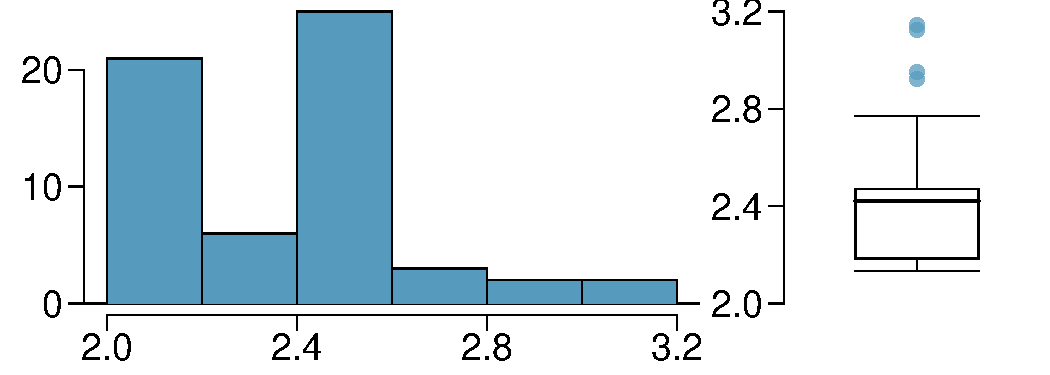
\includegraphics[width=0.6\textwidth]{ch_intro_to_data/figures/eoce/marathon_winners/marathon_winners_hist_box.pdf}
\end{center}
\begin{parts}
\item What features of the distribution are apparent in the histogram and not the box plot? What features are apparent in the box plot but not in the histogram?
\item What may be the reason for the bimodal distribution? Explain.
\item Compare the distribution of marathon times for men and women based on the box plot shown below.
\begin{center}
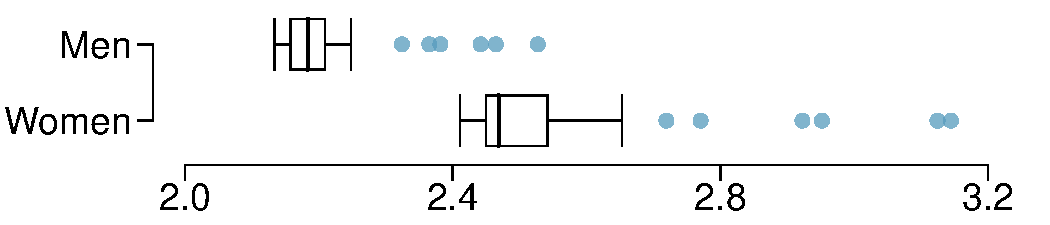
\includegraphics[width=0.6\textwidth]{ch_intro_to_data/figures/eoce/marathon_winners/marathon_winners_gender_box.pdf}
\end{center}
\item The time series plot shown below is another way to look at these data. Describe what is visible in this plot but not in the others.
\end{parts}
\begin{center}
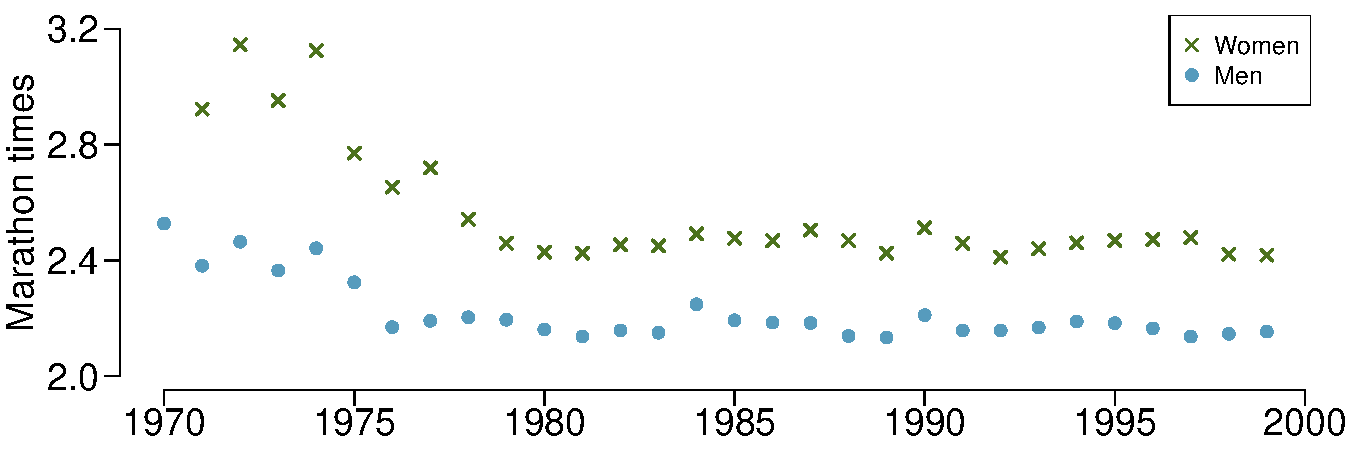
\includegraphics[width=0.75\textwidth]{ch_intro_to_data/figures/eoce/marathon_winners/marathon_winners_time_series.pdf} \\
\end{center}
}{}

\textC{\pagebreak}

% 55

\eoce{\qt{Distributions and appropriate statistics, Part I\label{dist_shape_pets_dist_height}} 
For each of the following, state whether you expect the distribution to be 
symmetric, right skewed, or left skewed. Also specify whether the mean or 
median would best represent a typical observation in the data, and whether 
the variability of observations would be best represented using the 
standard deviation or IQR. Explain your reasoning.
\begin{parts}
\item Number of pets per household. 
\item Distance to work, i.e. number of miles between work and home.
\item Heights of adult males.
\end{parts}
}{}

% 56

\eoce{\qt{Distributions and appropriate statistics, Part II
\label{dist_shape_housing_alcohol_salary}} For each of the following, state 
whether you expect the distribution to be symmetric, right skewed, or left skewed. 
Also specify whether the mean or median would best represent a typical observation 
in the data, and whether the variability of observations would be best represented 
using the standard deviation or IQR. Explain your reasoning.
\begin{parts}
\item Housing prices in a country where 25\% of the houses cost below \$350,000, 
50\% of the houses cost below \$450,000, 75\% of the houses cost below \$1,000,000 
and there are a meaningful number of houses that cost more than \$6,000,000.
\item Housing prices in a country where 25\% of the houses cost below \$300,000, 
50\% of the houses cost below \$600,000, 75\% of the houses cost below \$900,000 
and very few houses that cost more than \$1,200,000.
\item Number of alcoholic drinks consumed by college students in a given week. 
Assume that most of these students don't drink since they are under 21 years old, 
and only a few drink excessively.
\item Annual salaries of the employees at a Fortune 500 company where only a few 
high level executives earn much higher salaries than the all other employees.
\end{parts}
}{}

% 57

\eoce{\qt{TV watchers\label{dist_shape_TV_watchers}} Students in an AP Statistics class 
were asked how many hours of television they watch per week (including online 
streaming). This sample yielded an average of 4.71 hours, with a standard 
deviation of 4.18 hours. Is the distribution of number of hours students watch 
television weekly symmetric? If not, what shape would you expect this distribution 
to have? Explain your reasoning.
}{}

% 58

\eoce{\qt{Exam scores\label{dist_shape_exam_scores}} The average on a history exam 
(scored out of 100 points) was 85, with a standard deviation of 15. Is the 
distribution of the scores on this exam symmetric? If not, what shape would 
you expect this distribution to have? Explain your reasoning.
}{}

% 59

\eoce{\qt{Facebook friends\label{dist_shape_fb_friends}} Facebook data indicate that 
50\% of Facebook users have 100 or more friends, and that the average friend 
count of users is 190. What do these findings suggest about the shape of the 
distribution of number of friends of Facebook users? \footfullcite{Backstrom:2011}
}{}

% 60

\eoce{\qt{A new statistic\label{new_stat}} The statistic $\frac{\bar{x}}{median}$ can 
be used as a measure of skewness. Suppose we have a distribution where all 
observations are greater than 0, $x_i > 0$. What is the expected shape of 
the distribution under the following conditions? Explain your reasoning.
\begin{parts}
\item $\frac{\bar{x}}{median} = 1$
\item $\frac{\bar{x}}{median} < 1$
\item $\frac{\bar{x}}{median} > 1$
\end{parts}
}{}

\textC{\newpage}

% 61

\eoce{\qt{Income at the coffee shop\label{income_coffee_shop}} The first histogram 
below shows the distribution of the yearly incomes of 40 patrons at a college 
coffee shop. Suppose two new people walk into the coffee shop: one making 
\$225,000 and the other \$250,000. The second histogram shows the new income 
distribution. Summary statistics are also provided. \\
\begin{minipage}[c]{0.57\textwidth}
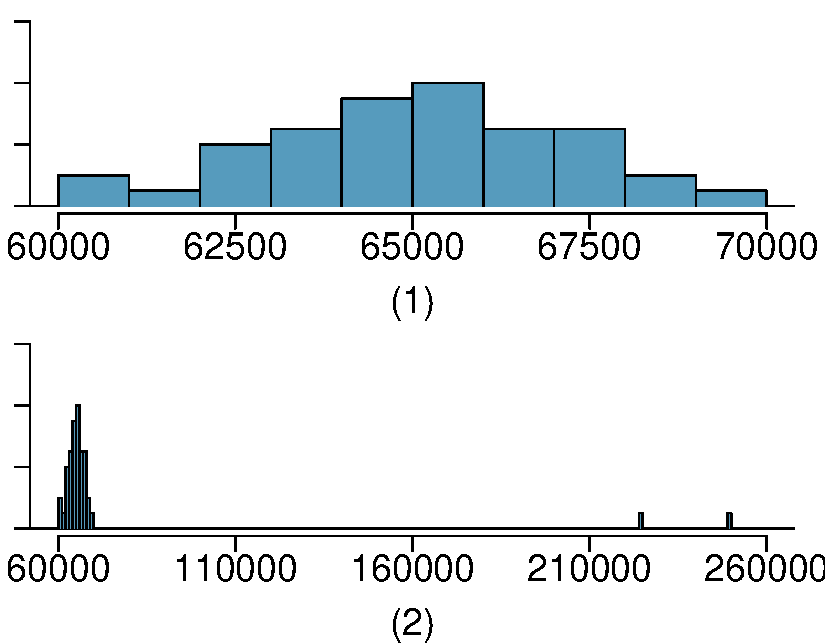
\includegraphics[width=\textwidth]{ch_intro_to_data/figures/eoce/income_coffee_shop/income_coffee_shop.pdf}
\end{minipage}
\begin{minipage}[c]{0.4\textwidth}
\begin{center}
\begin{tabular}{rrr}
\hline
        & (1)       & (2) \\ 
\hline
n       & 40        & 42 \\ 
Min.    & 60,680    & 60,680 \\ 
1st Qu. & 63,620    & 63,710 \\ 
Median  & 65,240    & 65,350 \\ 
Mean    & 65,090    & 73,300 \\ 
3rd Qu. & 66,160    & 66,540 \\ 
Max.    & 69,890    & 250,000 \\ 
SD      & 2,122     & 37,321 \\ 
\hline
\end{tabular}
\end{center}
\end{minipage}
\begin{parts}
\item Would the mean or the median best represent what we might think of as a 
typical income for the 42 patrons at this coffee shop? What does this say about 
the robustness of the two measures?
\item Would the standard deviation or the IQR best represent the amount of 
variability in the incomes of the 42 patrons at this coffee shop? What does 
this say about the robustness of the two measures?
\end{parts}
}{}

% 62

\eoce{\qt{Midrange\label{midrange}} The \textit{midrange} of a distribution is defined as 
the average of the maximum and the minimum of that distribution. Is this statistic 
robust to outliers and extreme skew? Explain your reasoning
}{}

% 63

\eoce{\qt{Commute times\label{county_commute_times}} The US census collects data on 
time it takes Americans to commute to work, among many other variables. The 
histogram below shows the distribution of average commute times in 3,143 US 
counties in 2010. Also shown below is a spatial intensity map of the same data.
\begin{center}
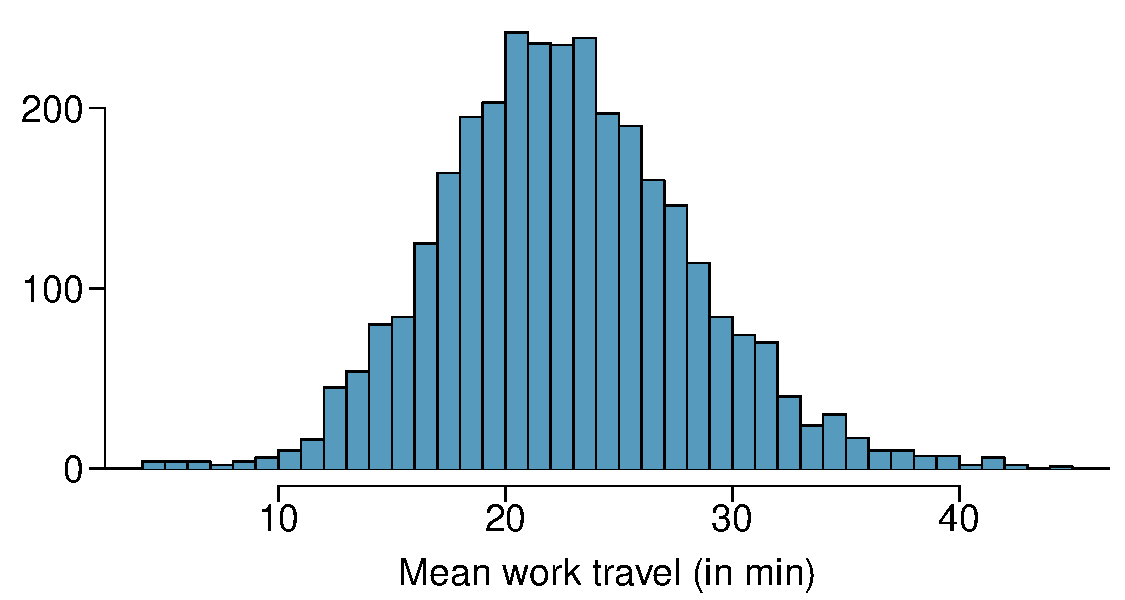
\includegraphics[width=0.48\textwidth]{ch_intro_to_data/figures/eoce/county_commute_times/county_commute_times_hist.pdf}
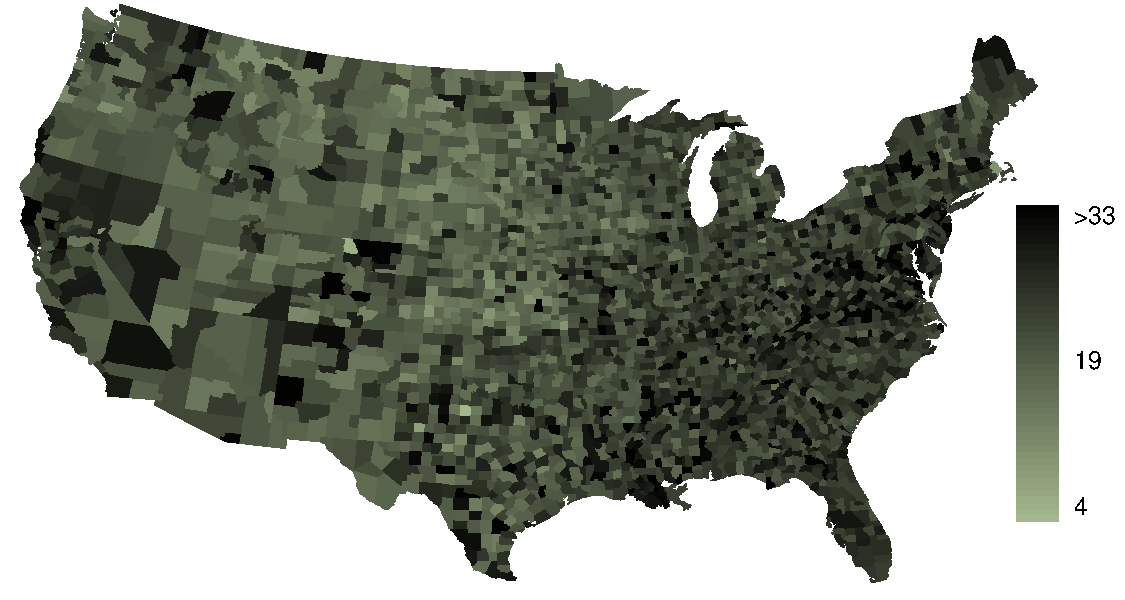
\includegraphics[width=0.48\textwidth]{ch_intro_to_data/figures/eoce/county_commute_times/county_commute_times_map.pdf}
\end{center}
\begin{parts}
\item Describe the numerical distribution and comment on whether or not a log 
transformation may be advisable for these data.
\item Describe the spatial distribution of commuting times using the map below.
\end{parts} 
}{}

\textC{\pagebreak}

% 64

\eoce{\qt{Hispanic population\label{county_hispanic_pop}} The US census collects 
data on race and ethnicity of Americans, among many other variables. The 
histogram below shows the distribution of the percentage of the population 
that is Hispanic in 3,143 counties in the US in 2010. Also shown is a 
histogram of logs of these values.
\begin{center}
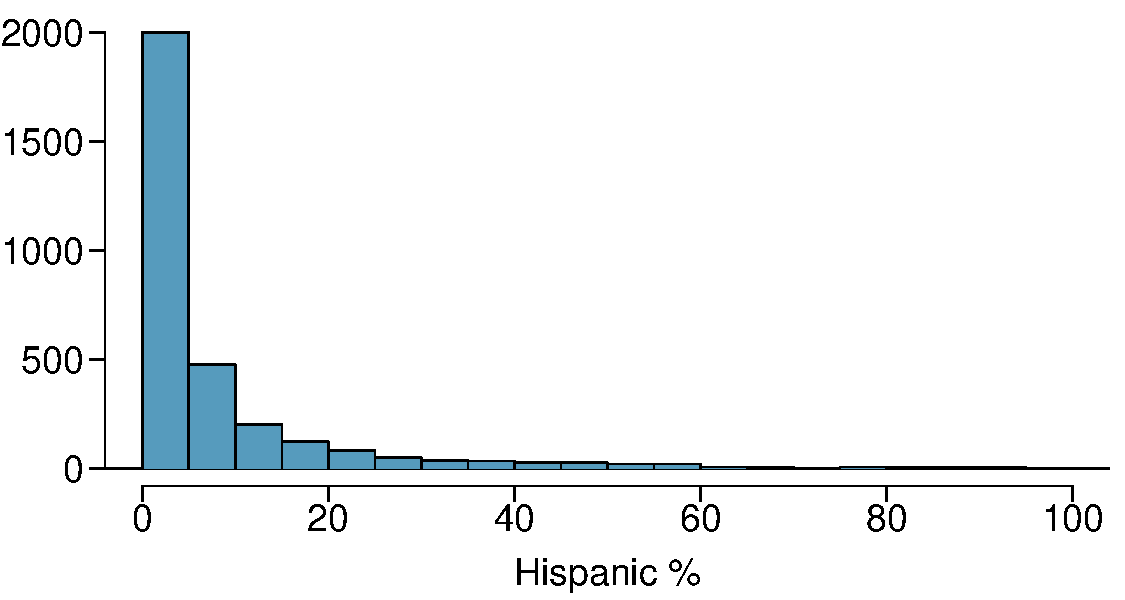
\includegraphics[width=0.48\textwidth]{ch_intro_to_data/figures/eoce/county_hispanic_pop/county_hispanic_pop_hist.pdf}
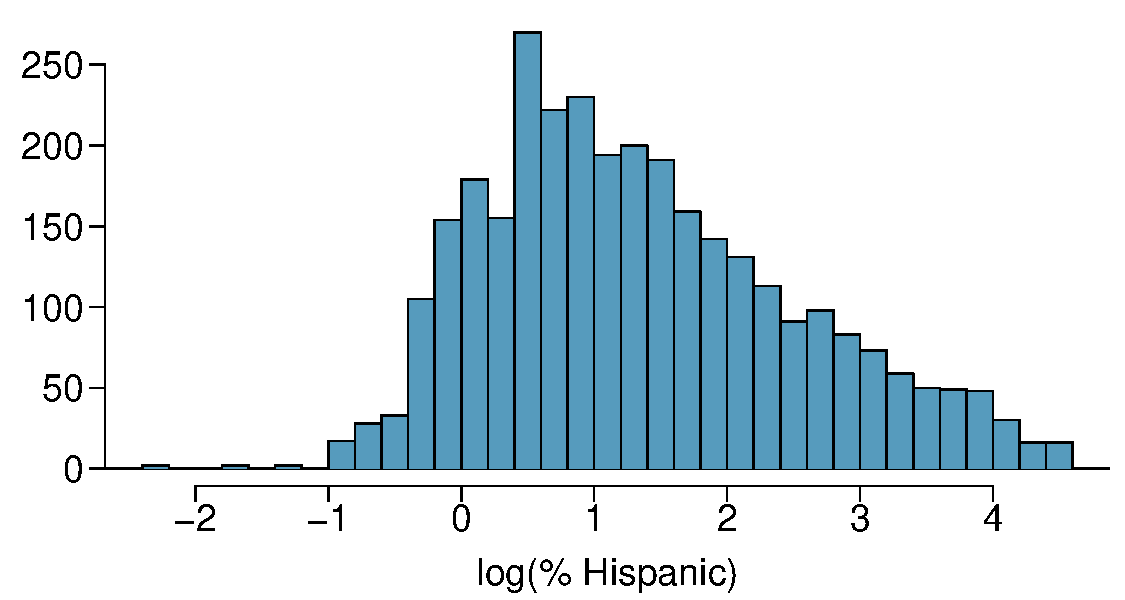
\includegraphics[width=0.48\textwidth]{ch_intro_to_data/figures/eoce/county_hispanic_pop/county_hispanic_pop_log_hist.pdf}
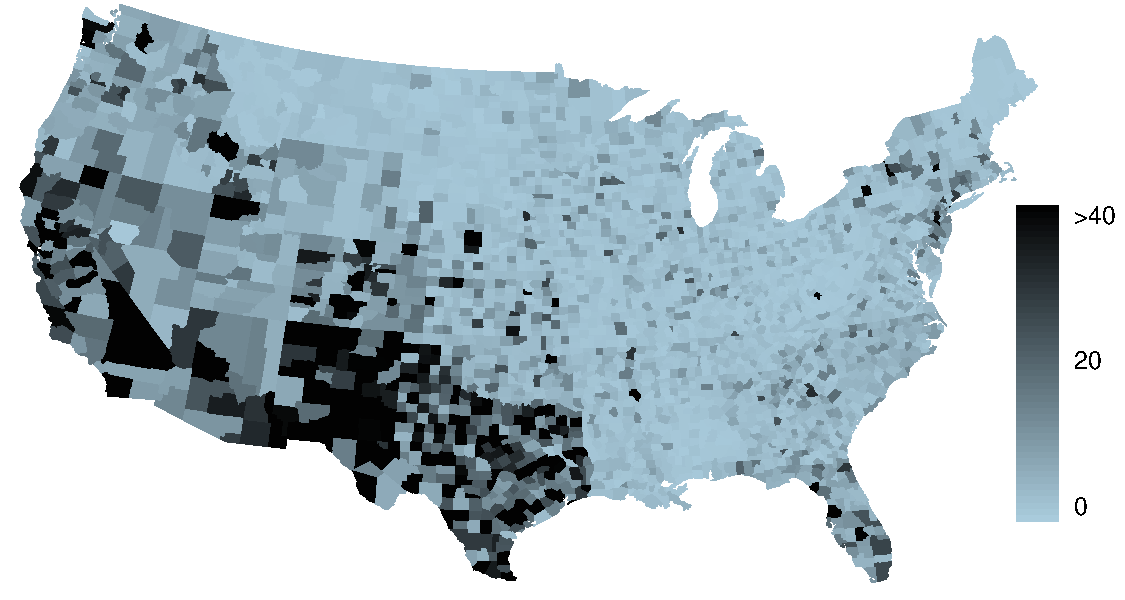
\includegraphics[width=0.48\textwidth]{ch_intro_to_data/figures/eoce/county_hispanic_pop/county_hispanic_pop_map.pdf}
\end{center}
\begin{parts}
\item Describe the numerical distribution and comment on why we might want 
to use log-transformed values in analyzing or modeling these data.
\item What features of the distribution of the Hispanic population in US 
counties are apparent in the map but not in the histogram? What features are 
apparent in the histogram but not the map?
\item Is one visualization more appropriate or helpful than the other? Explain 
your reasoning.
\end{parts} 
}{}


%_______________
\subsection{Considering categorical data}

% 65

\eoce{\qt{Antibiotic use in children\label{antibiotic_use_children}} The bar plot 
and the pie chart below show the distribution of pre-existing medical 
conditions of children involved in a study on the optimal duration of 
antibiotic use in treatment of tracheitis, which is an upper respiratory 
infection.
\begin{center}
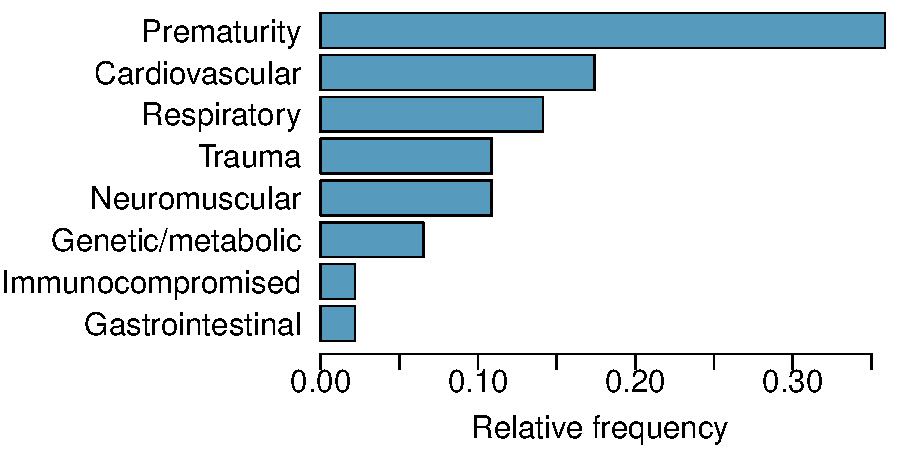
\includegraphics[width = 0.45\textwidth]{ch_intro_to_data/figures/eoce/antibiotic_use_children/antibiotic_use_children_bar}
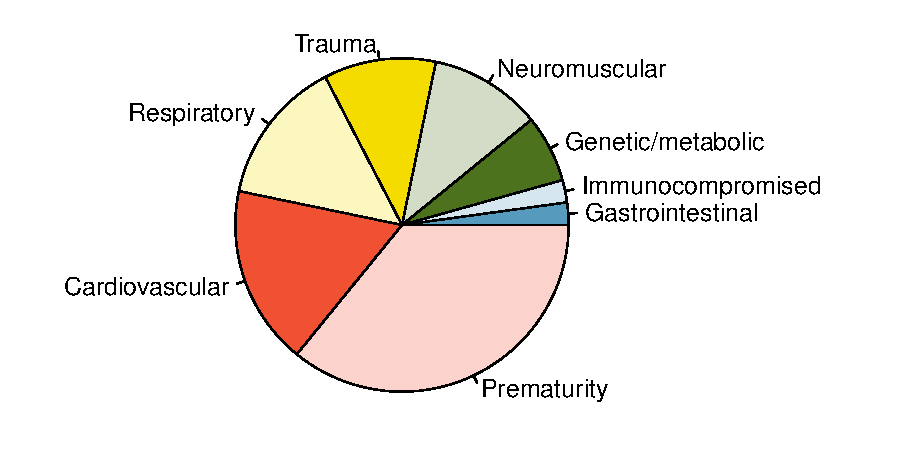
\includegraphics[width = 0.45\textwidth]{ch_intro_to_data/figures/eoce/antibiotic_use_children/antibiotic_use_children_pie}
\end{center}
\begin{parts}
\item What features are apparent in the bar plot but not in the pie chart?
\item What features are apparent in the pie chart but not in the bar plot?
\item Which graph would you prefer to use for displaying these categorical data?
\end{parts}
}{}

\textC{\pagebreak}

% 66

\eoce{\qt{Views on immigration\label{immigration}} 910 randomly sampled registered 
voters from Tampa, FL were asked if they thought workers who have illegally 
entered the US should be (i) allowed to keep their jobs and apply for 
US citizenship, (ii) allowed to keep their jobs as temporary guest workers 
but not allowed to apply for US citizenship, or (iii) lose their jobs and 
have to leave the country. The results of the survey by political ideology 
are shown below.\footfullcite{survey:immigFL:2012}
\begin{center}
\begin{tabular}{l l c c c c}
                        &                           & \multicolumn{3}{c}{\textit{Political ideology}} \\
\cline{3-5}
                        &                           & Conservative  & Moderate  & Liberal   & Total \\
\cline{2-6}
                        & (i) Apply for citizenship & 57            & 120       & 101       & 278 \\
                        & (ii) Guest worker         & 121           & 113       & 28        & 262 \\
\raisebox{1.5ex}[0pt]{\emph{Response}} & (iii) Leave the country    & 179       & 126       & 45        & 350 \\ 
                        & (iv) Not sure             & 15            & 4         & 1         & 20\\
\cline{2-6}
                        & Total                     & 372           & 363       & 175       & 910
\end{tabular}
\end{center}
\begin{parts}
\item What percent of these Tampa, FL voters identify themselves as conservatives?
\item What percent of these Tampa, FL voters are in favor of the citizenship option?
\item What percent of these Tampa, FL voters identify themselves as conservatives 
and are in favor of the citizenship option?
\item What percent of these Tampa, FL voters who identify themselves as 
conservatives are also in favor of the citizenship option? What percent of 
moderates share this view? What percent of liberals share this view?
\item Do political ideology and views on immigration appear to be independent? 
Explain your reasoning.
\end{parts}
}{}

% 67

\eoce{\qt{Views on the DREAM Act\label{dream_act_mosaic}} A random sample of registered 
voters from Tampa, FL were asked if they support the DREAM Act, a proposed law which would provide a path to citizenship for people brought illegally to the US as children.
The survey also collected information on the political ideology of the respondents. 
Based on the mosaic plot shown below, do views on the DREAM Act and  
political ideology appear to be independent? Explain your reasoning.
\footfullcite{survey:immigFL:2012}
\begin{center}
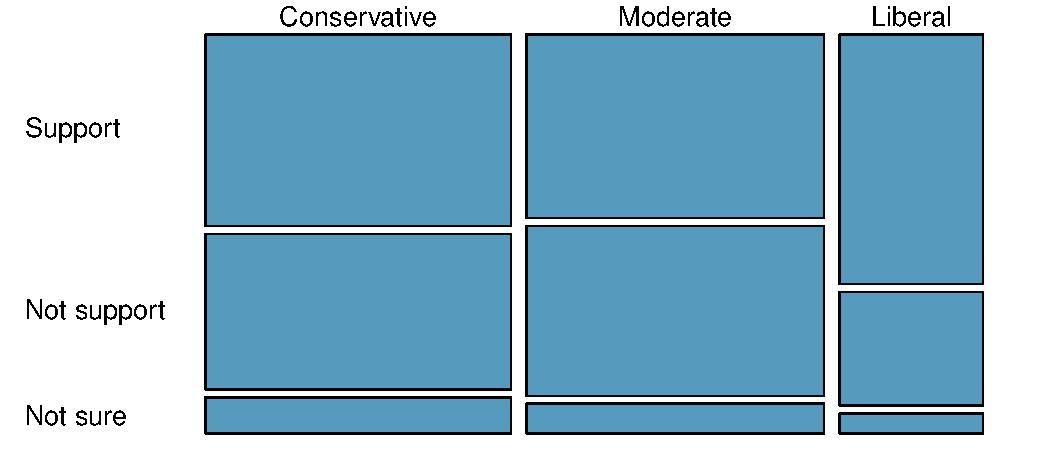
\includegraphics[width = 0.8\textwidth]{ch_intro_to_data/figures/eoce/dream_act_mosaic/dream_act_mosaic.pdf}
\end{center}
}{}

\textC{\newpage}

% 68

\eoce{\qt{Raise taxes\label{raise_taxes_mosaic}} A random sample of registered 
voters nationally were asked whether they think it's better to raise taxes 
on the rich or raise taxes on the poor. The survey also collected information 
on the political party affiliation of the respondents. Based on the mosaic 
plot shown below, do views on raising taxes and  
political affiliation appear to be independent? Explain your reasoning.
\footfullcite{survey:raiseTaxes:2015}
\begin{center}
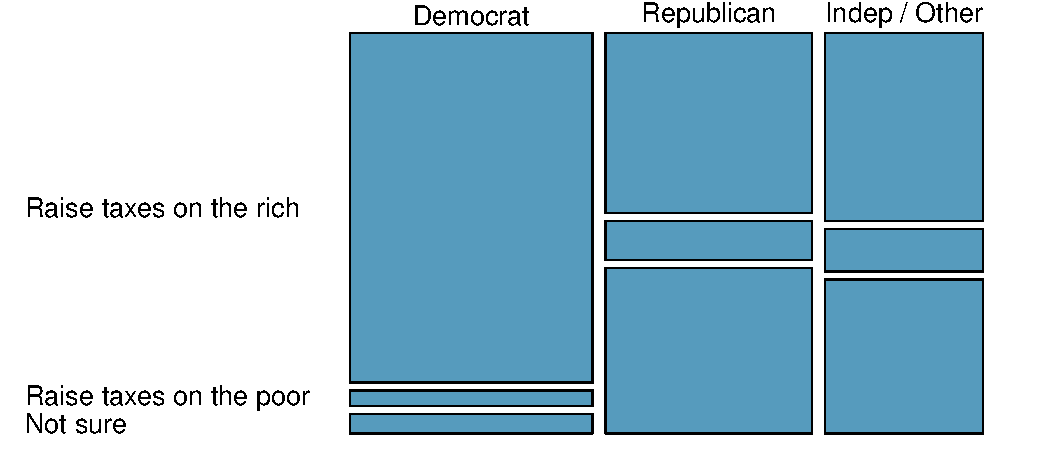
\includegraphics[width = 0.67\textwidth]{ch_intro_to_data/figures/eoce/raise_taxes_mosaic/raise_taxes_mosaic.pdf}
\end{center}
}{}


%_______________
\subsection{Case study: gender discrimination}

% 69

\eoce{\qt{Side effects of Avandia\label{randomization_avandia}} Rosiglitazone is the 
active ingredient in the controversial type~2 diabetes medicine Avandia and has 
been linked to an increased risk of serious cardiovascular problems such as 
stroke, heart failure, and death. A common alternative treatment is pioglitazone, 
the active ingredient in a diabetes medicine called Actos. In a nationwide 
retrospective observational study of 227,571 Medicare beneficiaries aged  
65 years or older, it was found that 2,593 of the 67,593 patients using 
rosiglitazone and 5,386 of the 159,978 using pioglitazone had serious 
cardiovascular problems. These data are summarized in the contingency 
table below. \footfullcite{Graham:2010}
\begin{center}
\begin{tabular}{ll  cc c} 
                                &   & \multicolumn{2}{c}{\textit{Cardiovascular problems}} \\
\cline{3-4} 
                                    &               & Yes   & No        & Total \\
\cline{2-5}
\multirow{2}{*}{\textit{Treatment}} & Rosiglitazone & 2,593 & 65,000    & 67,593 \\
                                    & Pioglitazone  & 5,386 & 154,592   & 159,978 \\
\cline{2-5}
                                    & Total         & 7,979 & 219,592   & 227,571
\end{tabular}
\end{center}
\begin{parts}
\item Determine if each of the following statements is true or false. If false, explain why. \textit{Be careful:} The reasoning may be wrong even if the statement's conclusion is correct. In such cases, the statement should be considered false.
\begin{subparts}
\item Since more patients on pioglitazone had cardiovascular problems (5,386 vs. 2,593), we can conclude that the rate of cardiovascular problems for those on a pioglitazone treatment is higher.
\item The data suggest that diabetic patients who are taking rosiglitazone are more likely to have cardiovascular problems since the rate of incidence was (2,593 / 67,593 = 0.038) 3.8\% for patients on this treatment, while it was only (5,386 / 159,978 = 0.034) 3.4\% for patients on pioglitazone.
\item The fact that the rate of incidence is higher for the rosiglitazone group proves that rosiglitazone causes serious cardiovascular problems.
\item Based on the information provided so far, we cannot tell if the difference between the rates of incidences is due to a relationship between the two variables or due to chance.
\end{subparts}
\textC{\textbf{(See the next page for additional parts to this question.)}}
\item What proportion of all patients had cardiovascular problems?
\item If the type of treatment and having cardiovascular problems were independent, about how many patients in the rosiglitazone group would we expect to have had cardiovascular problems?
\item We can investigate the relationship between outcome and treatment in this study using a randomization technique.  While in reality we would carry out the simulations required for randomization using statistical software, suppose we actually simulate using index cards. In order to simulate from the independence model, which states that the outcomes were independent of the treatment, we write whether or not each patient had a cardiovascular problem on cards, shuffled all the cards together, then deal them into two groups of size 67,593 and 159,978. We repeat this simulation 1,000 times and each time record the number of people in the rosiglitazone group who had cardiovascular problems. Use the relative frequency histogram of these counts to answer (i)-(iii).
\end{parts}
\begin{minipage}[c]{0.5\textwidth}
\begin{subparts}
\item What are the claims being tested?
\item Compared to the number calculated in part (b), which would provide more support for the alternative hypothesis,  \textit{more} or \textit{fewer} patients with cardiovascular problems in the rosiglitazone group?
\item What do the simulation results suggest about the relationship between taking rosiglitazone and having cardiovascular problems in diabetic patients?
\end{subparts}
\end{minipage}
\begin{minipage}[c]{0.5\textwidth}
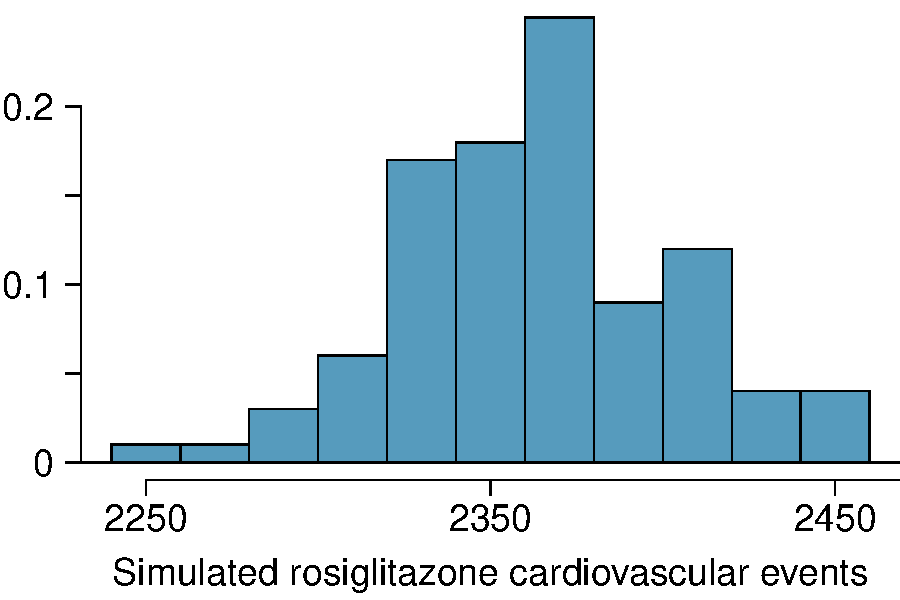
\includegraphics[width = \textwidth]{ch_intro_to_data/figures/eoce/randomization_avandia/randomization_avandia.pdf} \\
\end{minipage}
}{}

% 70

\eoce{\qt{Heart transplants\label{randomization_heart_transplants}} The Stanford 
University Heart Transplant Study was conducted to determine whether an 
experimental heart transplant program increased lifespan. Each patient 
entering the program was designated an official heart transplant candidate, 
meaning that he was gravely ill and would most likely benefit from a new heart. 
Some patients got a transplant and some did not. The variable \texttt{transplant} 
indicates which group the patients were in; patients in the treatment group got a 
transplant and those in the control group did not. Another variable called 
\texttt{survived} was used to indicate whether or not the patient was alive 
at the end of the study. Of the 34 patients in the control group, 30 died. Of the 69 people in the treatment group, 45 died. \footfullcite{Turnbull+Brown+Hu:1974}
\begin{center}
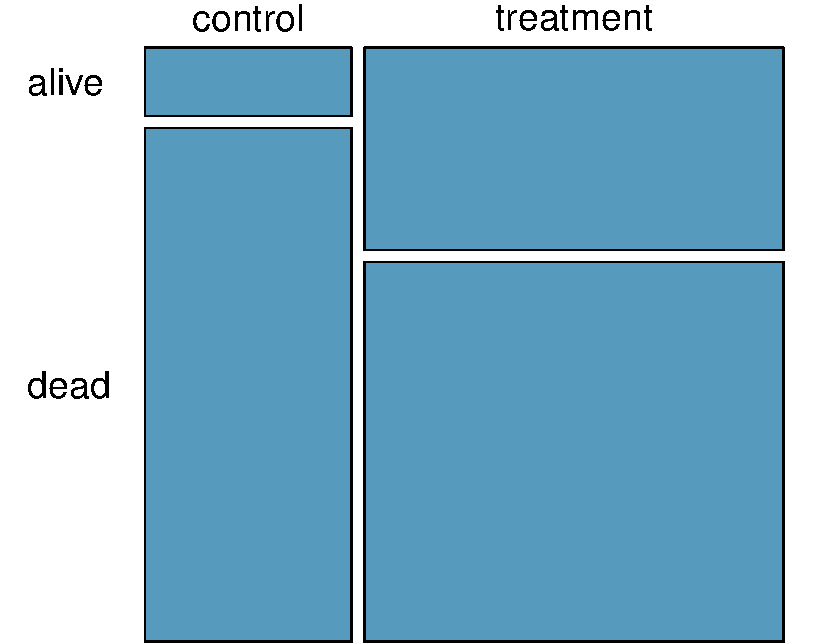
\includegraphics[width= 0.46\textwidth]{ch_intro_to_data/figures/eoce/randomization_heart_transplants/randomization_heart_transplants_mosaic.pdf}
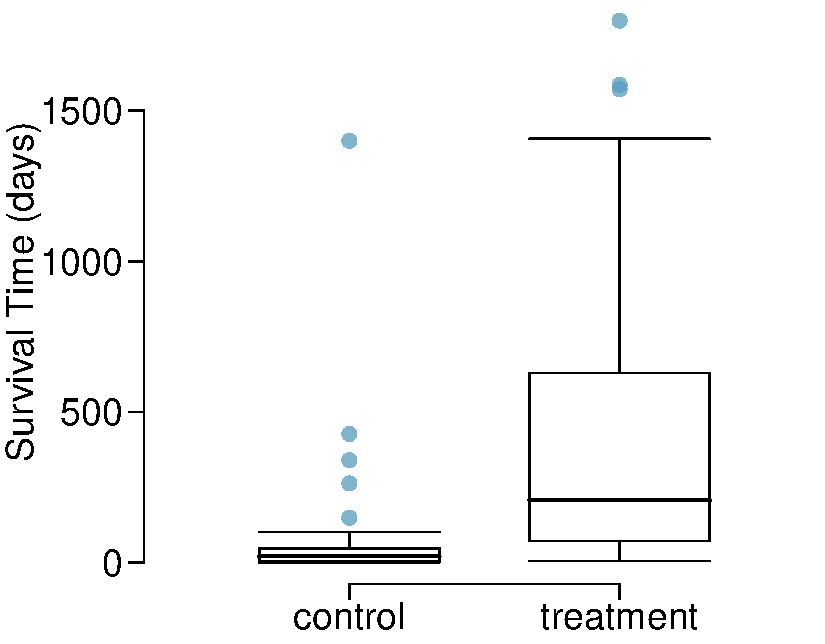
\includegraphics[width= 0.46\textwidth]{ch_intro_to_data/figures/eoce/randomization_heart_transplants/randomization_heart_transplants_box.pdf}
\end{center}
\begin{parts}
\item Based on the mosaic plot, is survival independent of whether or not the 
patient got a transplant? Explain your reasoning.
\textC{\\\textbf{(See the next page for additional parts to this question.)}}
\item What do the box plots below suggest about the efficacy (effectiveness) of the heart transplant treatment.
\item What proportion of patients in the treatment group and what proportion of 
patients in the control group died?
\item One approach for investigating whether or not the treatment is effective 
is to use a randomization technique.
\begin{subparts}
\item What are the claims being tested?
\item The paragraph below describes the set up for such approach, if we were 
to do it without using statistical software. Fill in the blanks with a number 
or phrase, whichever is appropriate.
\begin{adjustwidth}{2em}{2em}
We write \textit{alive} on \rule{2cm}{0.5pt} cards representing patients who were 
alive at the end of the study, and \textit{dead} on \rule{2cm}{0.5pt} cards 
representing patients who were not. Then, we shuffle these cards and split them 
into two groups: one group of size \rule{2cm}{0.5pt} representing treatment, and 
another group of size \rule{2cm}{0.5pt} representing control. We calculate the 
difference between the proportion of \textit{dead} cards in the treatment and 
control groups (treatment - control) and record this value. We repeat this 100 
times to build a distribution centered at \rule{2cm}{0.5pt}. Lastly, we calculate 
the fraction of simulations where the simulated differences in proportions are 
\rule{2cm}{0.5pt}. If this fraction is low, we conclude that it is unlikely to 
have observed such an outcome by chance and that the null hypothesis should 
be rejected in favor of the alternative.
\end{adjustwidth}
\item What do the simulation results shown below suggest about the effectiveness 
of the transplant program?
\end{subparts}
\end{parts}
\begin{center}
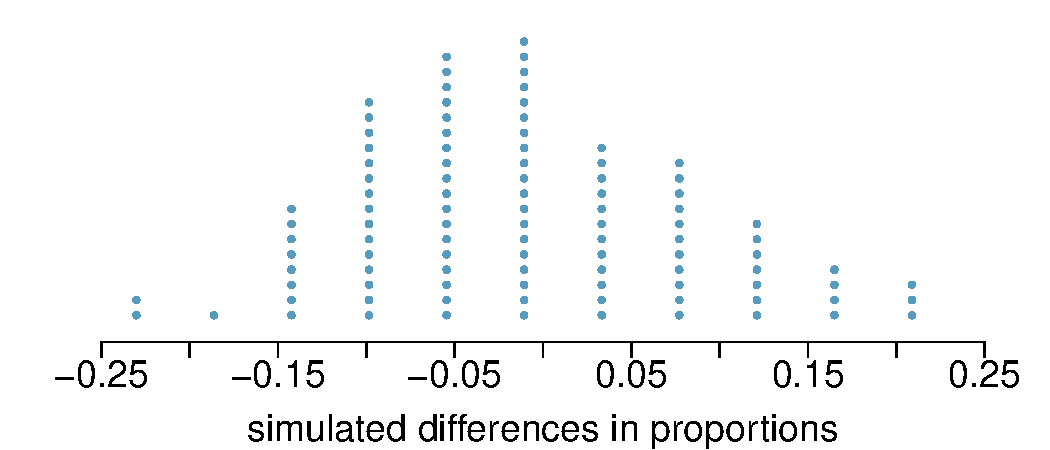
\includegraphics[width= 0.65\textwidth]{ch_intro_to_data/figures/eoce/randomization_heart_transplants/randomization_heart_transplants_rando.pdf}
\end{center}
}{}
